% ----- CHAPTER 5: ZERO SUMS ----- %

Algorithm \ref{algo:compute_rank} allows us to compute the rank of an elliptic curve in $\softO\left(\sqrt{N_E}\right)$ time by evaluating successive derivatives of $\Les$ at the central point. However, there is an inescapable limitation of this algorithm: the $\sqrt{N_E}$ time dependence of evaluating $\Les$ means that it becomes infeasible to run on modern computer hardware when the conductor is larger than about $10^{16}$. Moreover, since there is no known way to evaluate elliptic curve $L$-functions in faster than square-root-conductor time, there is essentially nothing we can do to make such a rank computation algorithm asymptotically faster. \\

In this section we work toward presenting a method to bound analytic rank from above that does not require direct computation of a curve's $L$-function. The upside of such an algorithm is that it can be run on curves with much larger conductor, with the tightness of the bound scaling with how long one wants computation time to be. The downside is that we will have to sacrifice exactness: the method will only provide upper bounds on rank. \\

Because the aforementioned method relies on sums over the zeros of $\Les$, for this entire section we will assume GRH unless explicitly stated otherwise.

\newpage
%%%%%%%%%%%%%%%%%%%%%%%%%%%%%%%%%%%%%%%%%%%%%%%%%%%%%%%%
\section{Logarithmic Derivatives}\label{sec:log_derivs}

Let $E/\QQ$  have conductor $N_E$.
\begin{definition}
The {\it logarithmic derivative} of the $L$-function attached to $E$ is
\begin{equation}
\ldLes := \frac{d}{ds} \log \Les = \frac{L_E^{\pr}(s)}{\Les}.
\end{equation}
\end{definition}
Logarithmic derivatives have some useful properties. Importantly, the logarithmic derivative of the product of meromorphic functions is the sum of the logarithmic derivatives thereof. To this end:
\begin{proposition}
\begin{equation}\label{eqn:logderiv_relation}
\ldLam{s} = \log\left(\frac{\sqrt{N_E}}{2\pi}\right) + \digamma(s) + \ldLe{s},
\end{equation}
where $\digamma(s) = \frac{\Gamma\pr}{\Gamma}(s)$ is the digamma function on $\C$.
\end{proposition}
This follows immediately from the definition of $\Lams = (N_E)^{\frac{s}{2}}(2\pi)^{-s}\Gamma(s)\Les$. \\

Note that the digamma function is well-understood and easily computable. It has simple poles at the negative integers, and it has the following infinite sum expansion about $s=1$:
\begin{equation}\label{eqn:digamma_sum}
\digamma(1+s) = -\eta + \sum_{k=1}^{\infty} \frac{s}{k(k+s)}.
\end{equation}
This series converges absolutely for any $s$ not equal to a negative integer, and uniformly on bounded sets (excluding the aforementioned negative integers).\\

What is perhaps surprising, however, is that $\ldLe{s}$ can be represented by an elegant Dirichlet series. Recall that for $p \nmid N_E$, the characteristic polynomial of Frobenius w.r.t.~$f$ at $p$ is $x^2 - a_p x + p^2$, where $a_p$ is as given by Definition \ref{def:a_p}. Let this quadratic polynomial split as $(x-\alpha_p)(x-\beta_p)$ in $\CC$, where for $\alpha_p$ and $\beta_p$ the dependence on $E$ is understood. \\

\begin{definition}\label{def:bn}
For $n \in \NN$, let
\begin{equation}
b_n(E) := \begin{cases}
-\left(\alpha_p^e+\beta_p^e\right)\cdot \log(p), & n=p^e\;\;\text{a prime power ($e\ge1$), and $p \nmid N_E$} \\
-a_p^e \cdot \log(p), & n=p^e\;\;\text{and $p \mid N_E$} \\
0, & \text{otherwise.} \end{cases}
\end{equation}
\end{definition}

\begin{lemma}
The Dirichlet series for $\ldLes$ is given by
\begin{equation}
\ldLes = \sum_{n=1}^{\infty} b_n(E)\, n^{-s},
\end{equation}
where the coefficients $b_n(E)$ are defined as in Definition \ref{def:bn}. \\
\end{lemma}
\begin{proof}
The proof is an exercise in taking the logarithmic derivative of the Euler product formula for $\Les$ and simplifying. Note we may write the Euler product of $\Les$ as
\begin{equation}
\Les = \prod_{p|N_E} \left(1-a_p p^{-s}\right)^{-1} \prod_{p\nmid N_E} \left(1-\alpha_p p^{-s}\right)^{-1}\left(1-\beta_p p^{-s}\right)^{-1}.
\end{equation}
The result follows by taking the logarithmic derivative of each term individually and then summing the results.
\end{proof}

The Dirichlet coefficients for $\ldLes$ have a beautiful characterization in terms of the number of points on $E$ over finite fields:
\begin{proposition}
\begin{equation}
b_n(E) = \begin{cases}
-\left(p^e + 1 - \#\widetilde{E}(\FF_{p^e})\right)\cdot \log(p), & n=p^e\;\;\text{a prime power,} \\
0, & \text{otherwise.} \end{cases}
\end{equation}
where $\#\widetilde{E}(\FF_{p^e})$ is the number of points over $\FF_{p^e}$ on the (possibly singular) curve obtained by reducing $E$ modulo $p$.
\end{proposition}

\begin{proof}
It is a standard result that if $(x-\alpha_p)(x-\beta_p)$ is the characteristic polynomial for Frobenius on $E$ for the prime of good reduction $p$, then
\begin{equation}
\#E(\FF_{p^e}) = p^e + 1 - \alpha_p^e - \beta_p^e
\end{equation}
(see \cite[pp. 134-136]{Sil-1985} for a proof), from which the result at $p \nmid N_E$ follows. \\

For primes of bad reduction, recall
\begin{equation}
a_p(E) := \begin{cases}
+1, & \text{$E$ has split multiplicative reduction at $p$} \\
-1, & \text{$E$ has non-split multiplicative reduction at $p$} \\
0, & \text{$E$ has additive reduction at $p$.}
\end{cases}
\end{equation}
Let $\Ensfpe$ be the group of nonsingular points on $\widetilde{E}(\FF_{p^e})$. \\
When $E$ has additive reduction at $p$, $\Ensfpe \simeq (\F_{p^e},+)$, so together with the singular point $\#\widetilde{E}(\FF_{p^e}) = p^e+1$; \\
Hence $(p^e + 1 - \#\widetilde{E}(\FF_{p^e}))\log(p) = 0 = a_p^e \log(p)$. \\
When $E$ has split multiplicative reduction at $p$, $\Ensfpe \simeq (\F_{p^e}^*,\times)$, so together with the singular point $\#\widetilde{E}(\FF_{p^e}) = (p^e-1)+1 = p^e$; So $(p^e + 1 - \#\widetilde{E}(\FF_{p^e}))\log(p) = 1\cdot \log(p) = a_p^e \log(p)$. \\
When $E$ has non-split multiplicative reduction at $p$, let $L/\FF_{p^e}$ be the quadratic extension obtained by adjoining to $\FF_{p^e}$ the slopes of the tangent lines  at the singular point; then $\Ensfpe \simeq \ker(\Norm_{L/\FF_{p^e}})$. \\
Some thought should convince you that there are $p^e-(-1)^e$ elements in $L$ with norm 1, so together with the singular point $\#\widetilde{E}(\FF_{p^e}) = p^e+1-(-1)^e$; \\
Hence $(p^e + 1 - \#\widetilde{E}(\FF_{p^e}))\log(p) = (-1)^e\cdot \log(p) = a_p^e \log(p)$.
See \cite[pg. 180, Prop. 5.1]{Sil-1985} for the proofs of the above isomorphisms.\\
\end{proof}

With elliptic curve $L$-functions it is often easier to work with the shifted logarithmic derivative $\ldLe{1+s}$ as it places the critical point at the origin. We therefore define notation for the coefficients of the shifted Dirichlet series below:
\begin{definition}\label{def:cn}
The logarithmic derivative of the shifted $L$-function $L_E(1+s)$ is given by Dirichlet series
\begin{equation}
\ldLe{1+s} := \sum_n c_n n^{-s} = \sum_{n} \frac{b_n}{n} n^{-s},
\end{equation}
i.e. $c_n = b_n/n$, where the $b_n$ are as defined in Definition \ref{def:bn}.
\end{definition}

Because of its transparent Dirichlet series, we can bound the magnitude of $\ldLe{1+s}$ for $\Re(s)>\frac{1}{2}$. Let $\frac{\zeta\pr}{\zeta}$ be the logarithmic derivative of the Riemann zeta function. Then $\frac{\zeta\pr}{\zeta}(s) = \sum -\Psi(n) n^{-s}$ for $\Re(s)>1$, where $\Psi(n)$ is the von Mangoldt function, given by
\begin{equation}\label{eqn:vonmangoldt}
\Psi(n) = \begin{cases} \log p & n = p^e \;\;\text{a perfect prime power,} \\ 0 & \text{otherwise.} \end{cases}
\end{equation}
(The von Mangoldt function is typically denoted $\Lambda(n)$ in the literature, but we have already reserved $\Lambda$ for the competed $L$-function of an elliptic curve). Observe that $-\frac{\zeta\pr}{\zeta}(s)$ is strictly positive for $s > 1$ real, and decays to zero exponentially as $s \to \infty$. \\

Away from the critical strip the behaviors of both $\Les$ and $\ldLe{s}$ are tightly constrained.
\begin{lemma}\label{lem:ldLe_bound}
Let $L_E(s)$ be the $L$-function of $E$. For any $s \in \CC$ with $\sigma := \Re(s) >\frac{3}{2}$, we have the following:
\begin{enumerate}
\item
\begin{equation}\label{ineq:bounds_on_Les}
\frac{\zeta(2\sigma-1)^2}{\zeta(\sigma-\frac{1}{2})^2} < \left|L_E(s)\right| < \zeta\left(\sigma-\frac{1}{2}\right)^2.
\end{equation}
\item
\begin{equation}\label{ineq:bounds_on_Ldles}
2\frac{\zeta\pr}{\zeta}\left(\sigma-\frac{1}{2}\right) < \left| \ldLe{s}\right| < -2\frac{\zeta\pr}{\zeta}\left(\sigma-\frac{1}{2}\right).
\end{equation}
\end{enumerate}
where $\zeta(s)$ is the Riemann Zeta function.
\end{lemma}

\begin{figure}[!h]
    \centering
    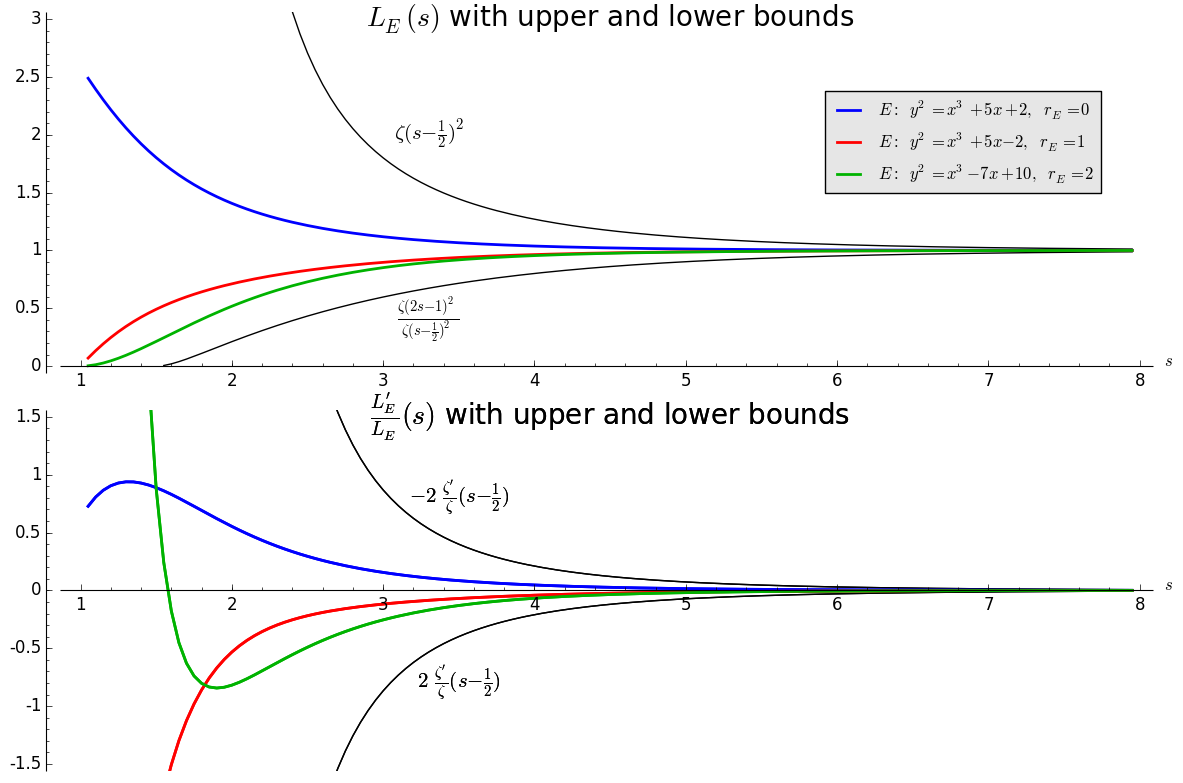
\includegraphics[width=1.0\textwidth]{graphics/L_E_and_logderiv_bounds.png}
    \caption{Plots of $L_E(s)$ and $\ldLes$ for $1<s<8$ for 3 elliptic curves -- one each of rank 0, 1 and 2 -- with the global bounds given in Lemma \ref{lem:ldLe_bound} drawn in.}
    \label{fig:L_E_and_logderiv_bounds}
\end{figure}

\begin{proof}
For the bound on $L_E(s)$, note that we may write the Euler product representation of $L_E(s)$ as
\begin{equation}
L_E(s) = \prod_{p \mid N_E} \left(\frac{1}{1-a_p p^{-s}}\right) \cdot \prod_{n \nmid N_E} \left(\frac{1}{1-\alpha_p p^{-s}}\right)\left(\frac{1}{1-\beta_p p^{-s}}\right),
\end{equation}
where for good $p$, $\alpha_p$ and $\beta_p$ are the two complex conjugate roots of the characteristic equation of Frobenius at $p$ for $E$. Hasse's Theorem has that these are both precisely $\sqrt{p}$ in magnitude; since $|a_p|\le 1$ for bad $p$ we thus derive the inequality
\begin{equation}
\prod_p \left(\frac{1}{1+ \sqrt{p}\cdot p^{-s}}\right)^2 < \left|L_E(s)\right| < \prod_p \left(\frac{1}{1- \sqrt{p}\cdot p^{-s}}\right)^2.
\end{equation}
We then note that 
\[ \prod_p \left(\frac{1}{1- \sqrt{p}\cdot p^{-s}}\right)^2 = \left(\prod_p \frac{1}{1- p^{-s+\frac{1}{2}}}\right)^2 = \zeta(s-\frac{1}{2})^2,\] 
while
\[ \prod_p \left(\frac{1}{1+ \sqrt{p}\cdot p^{-s}}\right)^2 = \left(\prod_p \frac{1- p^{-s+\frac{1}{2}}}{1- p^{-2s+1}}\right)^2 = \frac{\zeta(2s-1)^2}{\zeta(s-\frac{1}{2})^2}\]
to complete the result. \\ 

For the bound on $\ldLe{s}$, observe that Hasse's Theorem implies that $|q + 1 - \#\widetilde{E}(\FF_{q})| \le 2\sqrt{q}$ for any prime {\it power} $q$. Hence
\begin{align*}
\left| \ldLe{s}\right| &\le \sum_n |b_n| \cdot n^\sigma < \sum_{n} 2\sqrt{n} \cdot \lambda(n) n^{-\sigma}  = -2\frac{\zeta\pr}{\zeta}\left(\sigma-\frac{1}{2}\right).
\end{align*}
The left inequality is proved in the same way with the signs reversed. The resulting inequalities are indeed strict, as Hasse's bound is guaranteed not to be tight when, say, $p=2$.
\end{proof}
Note that these bounds are global: they do not depend on the elliptic curve $E$ in any way.

\begin{corollary}\label{cor:L_E_abs_convergence}
The Dirichlet series and Euler product for $L_E(s)$ converges absolutely for $\Re(s)>\frac{3}{2}$.
\end{corollary}
This follows immediately from the fact that $L_E(s)$ is bounded in magnitude by the $\zeta$ function shifted a half unit to the left, and the Dirichlet series for $\zeta(s)$ converges for $\Re(s)>1$.

\begin{corollary}
$\Lambda_E(1+s)$ has no zeros outside the critical strip $|\Re(s)| \le \frac{1}{2}$.
\end{corollary}
\begin{proof}
This may be proven via either set of inequalities in the above proposition; we will use the latter. Recall that if $f$ is meromorphic on $\CC$, then $\frac{f\pr}{f}$ has a pole at $s=s_0$ iff $f$ has a zero or pole at $s_0$; moreover poles of $\frac{f\pr}{f}$ are simple and have residue equal to the multiplicity of the corresponding zero/pole of $f$. But by the above $\ldLe{1+s}$ converges absolutely for $\Re(s)>\frac{1}{2}$, so $\ldLam{1+s}$ is well-defined and bounded for $\Re(s)>\frac{1}{2}$, and hence cannot have any poles in this region. By symmetry the same is true for $\Re(s)<-\frac{1}{2}$. Hence $\Lambda_E(1+s)$ cannot have any zeros for $|\Re(s)| > \frac{1}{2}$.
\end{proof}

If one assumes GRH, $\Lambda_E(1+s)$ has a particularly simple representation as a product over its zeros, from which we get a representation of $\ldLam{1+s}$ as a sum over its zeros.
\begin{proposition}[GRH]
\label{prop:logderiv_zero_rep} We have
\begin{enumerate}
\item \begin{equation}\label{eqn:Lams_prod}
\Lambda_E(1+s) = C_E\cdot s^{r_E} \cdot \prod_{\gamma > 0} \left(1+\frac{s^2}{\gamma^2}\right),
\end{equation}
where $C_E$ is the leading coefficient of $\Les$ at the central point (i.e. that defined in Conjecture \ref{conj:BSD}), and the product is taken over the imaginary parts of all nontrivial zeros of $\Lambda_E(1+s)$ in the upper half plane. The product converges absolutely for any $s$, and uniformly on any bounded set.
\item \begin{equation}\label{eqn:ldLam_sum}
\ldLam{1+s} = \sum_{\gamma} \frac{s}{s^2+\gamma^2}, 
\end{equation}
where the sum is taken over the imaginary parts of {\bf all} nontrivial zeros of $\Lambda_E(1+s)$, including central zeros with multiplicity. The sum converges absolutely for any $s$ outside the set of nontrivial zeros for $L_E(1+s)$, and uniformly on any bounded set outside of the set of zeros. \\
\end{enumerate}
\end{proposition}

Note that by GRH, $\gamma^2$ is always a nonnegative real number in any of the above expansions. Furthermore,  since noncentral nontrivial zeros occur in conjugate pairs, each term for $\gamma \ne 0$ in Equation \ref{eqn:ldLam_sum} appears exactly twice. It is therefore sometimes useful to rewrite it as
\begin{equation}\label{eqn:ldLam_sum_v2}
\ldLam{1+s} = \frac{r_E}{s} + 2 \sum_{\gamma>0} \frac{s}{s^2+\gamma^2},
\end{equation}
where $r_E$ is the (analytic) rank of $E$.

\begin{proof}
$\Lambda_E(1+s)$ has a zero of order $r_E$ at the origin, and by GRH all other zeros of $\Lambda_E(1+s)$ are simple, lie on the imaginary axis, and are symmetric about the origin. \\

Now since $\Lambda_E(1+s)$ is an entire function of finite order, we may express it as a Hadamard product over its zeros. As with the Hadamard product for the completed Riemann Zeta function, the symmetry of $\Lambda_E(1+s)$ simplifies this product to
\begin{equation}
\Lambda_E(1+s) = C_E \cdot s^{r_E}\cdot \prod_{\gamma\ne0}\left(1-\frac{s}{i\gamma}\right),
\end{equation}
where $C_E$ is the leading nonzero coefficient of the Taylor series for $\Lambda_E(1+s)$ at the central point; and for convergence the product should be taken over conjugate pairs of zeros. Combining conjugate pair terms yields Equation \ref{eqn:Lams_prod}; logarithmic differentiation then yields Equation \ref{eqn:ldLam_sum_v2}, which can be simplified to Equation \ref{eqn:ldLam_sum}.
\end{proof}

\begin{corollary}
$\ldLam{1+s}$ is an odd function.
\end{corollary}
Note this result holds independent of GRH. \\

Lemma \ref{lem:ldLe_bound} and Equation \ref{eqn:ldLam_sum} may be used to provide a crude bound on the analytic rank of $E$ with respect to its conductor:
\begin{corollary}\label{cor:logderiv_rank_bound}
Let $E$ have analytic rank $r_{an}(E)$ and conductor $N_E$. Then
\begin{equation}
r_{an}(E) < 1.6 + \frac{1}{2} \log N_E.
\end{equation}
Moreover, this bound is {\it unconditional}; it does not require GRH to hold.
\end{corollary}
\begin{proof}
We begin by assuming GRH. From Equation \ref{eqn:ldLam_sum} we have the point estimate
\begin{equation}\label{eqn:r_an_point_estimate}
r_{an} < \sum_{\gamma} \frac{1}{1+\gamma^2} = \ldLam{2},
\end{equation}
while from Lemma \ref{lem:ldLe_bound} we get
\begin{equation}
\ldLam{2} =  \log\left(\frac{\sqrt{N_E}}{2\pi}\right) + \digamma(2) + \ldLe{2} < \frac{1}{2}\log N_E  - \log 2\pi + 1-\eta -2\frac{\zeta\pr}{\zeta}\left(\frac{3}{2}\right),
\end{equation}
where $\digamma(s)$ is the digamma function on $\CC$ and $\eta$ is the Euler-Mascheroni constant $= 0.5772156649\ldots$. Collect constant terms and round up to get the stated bound. \\

If one does not assume GRH, then we must use a less simplified representation for the logarithmic derivative:
\begin{equation}
\ldLam{1+s} = \sum_{\rho} \frac{1}{2}\left( \frac{1}{s-\rho} + \frac{1}{s-\bar{\rho}}\right),
\end{equation}
where $\rho$ ranges over the nontrivial zeros of $L_E(1+s)$. However, everything else proceeds as before, and the point estimate given in Equation \ref{eqn:r_an_point_estimate} still holds.
\end{proof}
We will later use a related technique to show firstly that the factor in front of $\log N_E$ can be made arbitrarily small, at the expense of having to assume GRH and having to increase the added constant. \\

The following corollary of Proposition \ref{prop:logderiv_zero_rep} will be of import in obtaining explicit bounds on the number of zeros of $L_E(s)$ in a given interval on the critical strip:
\begin{corollary}[GRH]\label{cor:Re_logderiv}
Let $\Re(s) > 0$, and write $s = \sigma + i\tau$, i.e. $\sigma > 0$. Then
\begin{equation}
\sum_{\gamma} \frac{\sigma}{\sigma^2+(\gamma-\tau)^2} = \Re\left(\ldLam{1+s}\right),
\end{equation}
where again the sum is taken over all nontrivial zeros of $L_E(s)$. The sum converges absolutely for any $\tau \in \RR$ and $\sigma > 0$.
\end{corollary}
\begin{proof}
By equation \ref{eqn:ldLam_sum} we have
\begin{align*}
\Re\left(\ldLam{1+s}\right) &= \Re\left(\sum_{\gamma} \frac{s}{s^2+\gamma^2}\right) \\
& = \frac{1}{2} \sum_{\gamma} \Re\left(\frac{1}{s - i \gamma} + \frac{1}{s + i \gamma}\right) \\
&= \frac{1}{2} \sum_{\gamma} \frac{\sigma}{\sigma^2+(\gamma-\tau)^2} +  \frac{\sigma}{\sigma^2+(\gamma+\tau)^2}.
\end{align*}
However, absolute convergence for $\sum_{\gamma} \frac{s}{s^2+\gamma^2}$ for any $s$ in the right half plane implies absolute convergence for the individual sums $\sum_{\gamma} \frac{\sigma}{\sigma^2+(\gamma-\tau)^2}$ and $\sum_{\gamma} \frac{\sigma}{\sigma^2+(\gamma+\tau)^2}$. We may thus write
\begin{align*}
\Re\left(\ldLam{1+s}\right) &= \frac{1}{2} \sum_{\gamma} \frac{\sigma}{\sigma^2+(\gamma-\tau)^2} +  \frac{1}{2} \sum_{\gamma}\frac{\sigma}{\sigma^2+(\gamma+\tau)^2} \\
&= \sum_{\gamma} \frac{\sigma}{\sigma^2+(\gamma-\tau)^2} \;\;\text{by symmetry.}
\end{align*}
\end{proof}
Observe that GRH implies that $\Re(\ldLam{1+s})>0$ for $\Re(s)>0$, since then each of the terms in the above sum are strictly positive. By oddness of $\ldLam{1+s}$ we also then have that $\Re(\ldLam{1+s})<0$ for all $\Re(s)<0$, and $\Re(\ldLam{1+s})=0 \Rightarrow \Re(s)=0$. \\

\newpage
%%%%%%%%%%%%%%%%%%%%%%%%%%%%%%%%%%%%%%%%%%%%%%%%%%%%%%%%
\section{The Explicit Formula for Elliptic Curves}

Combining equations \ref{eqn:logderiv_relation}, \ref{eqn:digamma_sum} and \ref{eqn:ldLam_sum} we get the following equality:
\begin{proposition}[GRH]
Let $E/\QQ$ have conductor $N_E$. Let $\gamma$ range over all nontrivial zeros of $\Les$ with multiplicity, let $\eta$ be the Euler-Mascheroni constant, and let the $c_n = c_n(E)$ be as given by definitions \ref{def:bn} and \ref{def:cn}. Then
\begin{equation}\label{eqn:exp_form_1}
\sum_{\gamma} \frac{s}{s^2 + \gamma^2} = \left[-\eta + \log\left(\frac{\sqrt{N_E}}{2\pi}\right)\right] + \sum_{k=1}^{\infty} \frac{s}{k(s+k)} + \sum_{n=1}^{\infty} c_n n^{-s}.
\end{equation}
\end{proposition}
This is the prototypical {\it explicit formula} for elliptic curves: an equation relating a sum over the nontrivial zeros of $\Les$ to a sum over the logarithmic derivative coefficients of $\Les$, plus some easily smooth part that only depends on the curve's conductor. \\

In general, the phrase ``explicit formula" is not applied to a specific equation, but rather to a suite of equalities that resemble the above in some way. We reproduce Lemma 2.1 from \cite{Bob-2011}, which is a more general version of the explicit formula, akin to the Weil formulation of the Riemann-von Mangoldt explicit formula for $\zeta(s)$.
\begin{lemma}[GRH]
\label{lem:exp_form_2}
Suppose that $f(z)$ is an entire function s.t. there exists a $\delta>0$ such that $f(x+iy) = O(x^{-(1+\delta)})$ for $|y|<1+\epsilon$ for some $\epsilon>0$. Suppose that the Fourier transform of $f$
\begin{equation}
\hat{f}(y) = \int_{-\infty}^{\infty} e^{-i x y}f(x)\; dx
\end{equation}
exists and is such that $\sum_{n=1}^{\infty} c_n \hat{f}\left(\log n\right)$ converges absolutely. Then
\begin{equation}\label{eqn:exp_form_2}
\sum_{\gamma} f(\gamma) = \frac{1}{\pi}\left[\log\left(\frac{\sqrt{N_E}}{2\pi}\right)\hat{f}(0) + \Re\int_{-\infty}^{\infty} \digamma(1+it)f(t) \; dt  + \frac{1}{2} \sum_{n=1}^{\infty} c_n \left( \hat{f}\left(\log n\right) + \hat{f}\left(-\log n\right)\right) \right].
\end{equation}
\end{lemma}
A proof can be found in \cite[Theorem 5.12]{IwKo-2004}. Note that Equation \ref{eqn:exp_form_1} can be recovered by setting $f$ to be the Poisson kernel $f_s(x) = \frac{s}{s^2+x^2}$; then $\hat{f_s}(y) = e^{-s|y|}$, so $\hat{f_s}(\log n) = n^{-s}$. \\

We give a distribution-theoretic reformulation of Lemma \ref{lem:exp_form_2}. While the subject of explicit formulae for $L$-functions of Hecke eigenforms is treated by a number of sources, the following doesn't seem to have been explicitly written down in the literature anywhere:
\begin{proposition}[GRH]\label{prop:exp_form_as_distribution}
Let $\gamma$ range over the imaginary parts of the zeros of $\Les$ with multiplicity. Let $\varphi_E = \sum_{\gamma} \delta(x-\gamma)$ be the complex-valued distribution on $\RR$ corresponding to summation over the zeros of $L_E(s)$, where $\delta(x)$ is the usual Dirac delta function. That is, for any test function $f: \RR \mapsto \CC$ such that $\sum_{\gamma}f(\gamma)$ converges, 
\begin{equation}
\langle f,\varphi_E \rangle = \int_{-\infty}^{\infty} f(x)\left(\sum_{\gamma\in S_E} \delta(x-\gamma)\right) \, dx = \sum_{\gamma\in S_E} f(\gamma).
\end{equation}
Then as distributions,
\begin{equation}\label{eqn:exp_form_3}
\varphi_E = \sum_{\gamma} \delta(x-\gamma) = \frac{1}{\pi}\left[-\eta + \log\left(\frac{\sqrt{N_E}}{2\pi}\right) +\sum_{k=1}^{\infty} \frac{x^2}{k(k^2+x^2)} + \frac{1}{2}\sum_{n=1}^{\infty} c_n \left(n^{ix}+n^{-ix}\right) \right].
\end{equation}
\end{proposition}
In the above language, $\ldLam{1+s} = \left\langle \frac{s}{s^2+x^2},\varphi_E \right\rangle$ for $\Re(s) > 0$. Note that convergence on the right hand side is absolute for $\Re(s)>1$, and conditional (provably so thanks to Sato-Tate) for $0<\Re(s)\le 1$. \\

\newpage
%%%%%%%%%%%%%%%%%%%%%%%%%%%%%%%%%%%%%%%%%%%%%%%%%%%%%%%%
\section{Estimating Analytic Rank with the sinc$^2$ Sum}\label{sec:sinc_squared_sum}

The Explicit Formula may be used to provide computationally effective upper bounds on the analytic rank of an elliptic curve. The method appears to have first been formulated by Mestre in \cite{Me-1986}, and used by Brumer in \cite{Bru-1992} to prove that, conditional on GRH, the average rank of elliptic curves was at most 2.3. This upper bound was improved to 2 by Heath-Brown in \cite{HeBr-2004}. \\

[Aside: one of the most groundbreaking developments in number theory in recent years is a series of results by Manjul Bhargava and Arul Shankar \cite{BhSh-2010a} \cite{BhSh-2010b} \cite{BhSh-2013} proving that the average rank of elliptic curves is at most 0.885. These results are {\it unconditional}; the first such unconditional bound on average rank. For his work Bhargava received a Fields Medal in 2014.] \\

The analytic method stems from invoking the explicit formula as stated in Lemma \ref{lem:exp_form_2} on a function $f$ of a specific form:
\begin{lemma}[GRH]\label{lem:exp_form_nonneg_f_cpt_suppt}
Let $\gamma$ range over the nontrivial zeros of $L_E(s)$. Let $f$ be a non-negative even real-valued function on $\RR$ such that $f(0)=1$. Suppose further that the Fourier transform $\hat{f}$ of $f$ has compact support, i.e. $\hat{f}(y) = 0$ for $|y|>R$ for some $R>0$. Then for any $\Delta>0$, we have
\begin{equation}
\sum_{\gamma} f(\Delta \gamma) = \frac{1}{\Delta \pi}\log\left(\frac{\sqrt{N_E}}{2\pi}\right) + \Re\int_{-\infty}^{\infty} \digamma(1+it)f(\Delta t) \; dt  + \frac{1}{\Delta \pi}\sum_{n<e^{\Delta R}} c_n \hat{f}\left(\frac{\log n}{\Delta}\right).
\end{equation}
Moreover, the value of the sum bounds from above the analytic rank of $E$ for any given value of $\Delta$, and sum converges to $r_{\an}(E)$ as $\Delta \to \infty$.
\end{lemma}

\begin{proof}
The formula as stated above is just an application of the explicit formula in Lemma \ref{lem:exp_form_2}, noting that the Fourier transform of $f(\Delta x)$ is $\frac{1}{\Delta}\hat{f}\left(\frac{\xi}{\Delta}\right)$. Since $f$ is $1$ at the origin, $\sum_{\gamma} f(\Delta \gamma) = r_E + \sum_{\gamma\ne 0} f(\Delta \gamma)$. Furthermore, $f$ is non-negative and integrable, so the sum over noncentral zeros is nonnegative and decreases to zero as $\Delta$ increases.
\end{proof}

While in theory any $f$ with the properties mentioned above work for bounding analytic rank, the function
\begin{equation}
f(x) = \sinc^2(x) = \left(\frac{\sin(\pi x)}{\pi x}\right)^2
\end{equation}
is what is used by Mestre, Brumer, Heath-Brown in the publications above, and by Bober in \cite{Bob-2011}. This is due to its Fourier transform being compactly supported, namely is the triangular function:
\begin{equation}
\hat{f}(y) = \int_{-\infty}^{\infty} e^{-i x y}f(x)\; dx =  \begin{cases} 1 - \frac{|y|}{2\pi}, & |y|\le 2\pi \\ 0, & |y| > 2\pi.\end{cases}
\end{equation}
Moreover, if $f(x) = \sinc^2(x)$, the integral $\Re\int_{-\infty}^{\infty} \digamma(1+it)f(\Delta t) \; dt$ can be computed explicitly in terms of known constants and special functions:
\begin{equation}
\Re\int_{-\infty}^{\infty} \digamma(1+it)f(\Delta t) \; dt = - \frac{\eta}{\pi \Delta} + \frac{1}{2\pi^2 \Delta^2}\left(\frac{\pi^2}{6} - \Li_2\left(e^{-2\pi \Delta}\right)\right),
\end{equation}
where $\eta$ is the Euler-Mascheroni constant $= 0.5772\ldots$ and $\Li_2(x)$ is the dilogarithm function, defined as $\Li_2(x) = \sum_{k=1}^{\infty} \frac{x^k}{k^2}$ for $|x|\le 1$.

Combining the above, we get a specialization of Lemma \ref{lem:exp_form_nonneg_f_cpt_suppt}:
\begin{corollary}[GRH]
Let $\gamma$ range over the nontrivial zeros of $L_E(s)$, and let $\Delta > 0$. Then
\begin{align}\label{eqn:sincsquared_sum}
\sum_{\gamma} \sinc^2(\Delta \gamma) = \quad &\frac{1}{\Delta \pi}\left[\left(-\eta + \log\left(\frac{\sqrt{N_E}}{2\pi}\right)\right)+ \frac{1}{2\pi \Delta}\left(\frac{\pi^2}{6} - \Li_2\left(e^{-2\pi \Delta}\right)\right)  \right. \nonumber \\
&+ \left.\sum_{n<e^{2\pi \Delta}} c_n \cdot \left(1-\frac{\log n}{2\pi \Delta}\right)\right].
\end{align}
\end{corollary}

What's notable about the above formula is that evaluation of the right hand side is a finite computation, and only requires knowledge of the elliptic curve's conductor and its $a_p$ values up to some bound. Thus the zero sum is eminently computable, and results in a value that bounds from above the analytic rank of $E$. \\

\begin{figure}[!h]
    \centering
    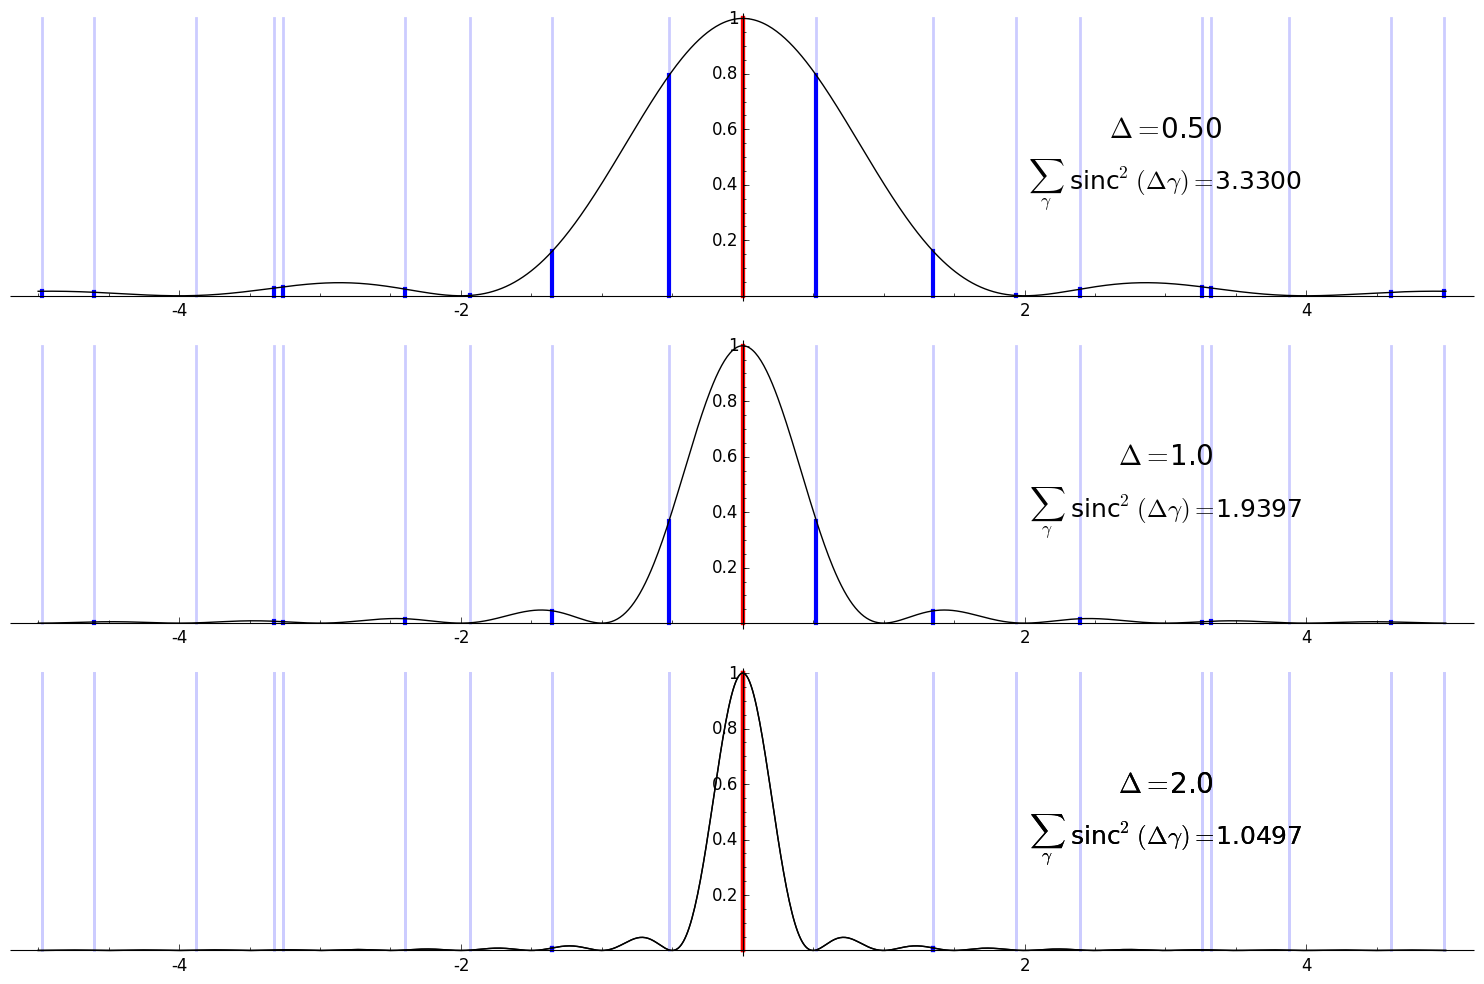
\includegraphics[width=1.0\textwidth]{graphics/zero_sum_visualization.png}
    \caption{A graphic representation of the $\sinc^2$ sum for the elliptic curve $E: y^2=x^3-18x+51$, a rank 1 curve with conductor $N_E=750384$, for three increasing values of the parameter $\Delta$. Vertical lines have been plotted at $x=\gamma$ whenever $L_E(1+i\gamma)=0$ -- red for the single central zero, and blue for noncentral zeros; the height of the darkened portion of each line is given by the black curve $\sinc^2(\Delta x)$. Summing up the lengths of the dark vertical lines thus gives the value of the $\sinc^2$ sum. We see that as $\Delta$ increases, the contribution from the blue lines -- corresponding to noncentral zeros -- goes to zero, while the contribution from the central zero in red remains at 1. Thus the sum must limit to 1 as $\Delta$ increases.}
    \label{fig:zero_sum_visualization}
\end{figure}

The $\sinc^2$ zero sum rank estimation method has been implemented in Sage (see Appendix A), and used to successfully estimate ranks on a database of 18 million elliptic curves with conductor at most $\sim 10^{11}$. A range of $\Delta$ values was used, from $\Delta=1.0$ (for which average time per curve was $\sim 10^{-5}$ s), to $\Delta=2.0$ (average time per curve $\sim 10^{-1}$ s). See an upcoming paper by Ho, Balakrishnan, Kaplan, Stein, Weigandt, and S. for details on the computations. \\

A neat conclusion that can immediately be drawn from the finiteness of the $\sinc^2$ explicit formula sum, is that maximum analytic rank grows more slowly than $\log N_E$:

\begin{corollary}[GRH]\label{cor:rank_slower_than_log_N}
For any $\epsilon >0$ there is a constant $K_{\epsilon}>0$ such that for any $E/\QQ$ with conductor $N_E$, we have
\begin{equation}
r_E < \epsilon \log N_E + K_{\epsilon}.
\end{equation}
\end{corollary}
\begin{proof}
We note that for any given $\Delta>0$, the sum $ \sum_{n<e^{2\pi \Delta}} c_n \cdot \left(1-\frac{\log n}{2\pi \Delta}\right)$ is bounded by a constant that is independent of the choice of elliptic curve, as the $c_n$ values are bounded globally. Thus the right hand side of Equation \ref{eqn:sincsquared_sum} is equal to $\frac{1}{2\pi \Delta}\log N_E$ plus a number whose supremum magnitude depends only on $\Delta$ and not on $E$. Since the sum bounds analytic rank, taking $\epsilon = \frac{1}{2\pi \Delta}$ and letting $\epsilon \to 0$ proves the statement.
\end{proof}

[Aside: This statement is already known in the literature, so nothing new has been proven here. In fact, it's conjectured that maximum analytic rank grows more like $\sqrt{\log N_E}$ (existing numerical evidence would seem to support this), but this is still very much an open problem.] \\

The above allows us to provide bounds on analytic rank via point estimates by choosing particular values of $\epsilon$. For example, if we choose $\epsilon = \frac{1}{\log 23} \sim 0.3189\ldots$ and collect and bound all the conductor-independent terms in equation \ref{eqn:sincsquared_sum}, we can improve the result in Corollary \ref{cor:logderiv_rank_bound} to the following:
\begin{corollary}[GRH]\label{cor:better_an_bound}
Let $E$ have analytic rank $r_E$ and conductor $N_E$. Then
\begin{equation}
r_E < 0.32 \log N_E + 0.5.
\end{equation}
\end{corollary}
We leave the details of the proof to the reader as a fun analysis exercise.\\

Finally, it's worth noting is that when $\Delta \le \frac{\log 2}{2\pi}$, the $c_n$ sum in Equation \ref{eqn:sincsquared_sum} is empty. Thus we have the following:
\begin{corollary}[GRH]
Let $E/\QQ$ have conductor $N_E$. Let $\eta$ be the Euler-Mascheroni constant $=0.5772\ldots$, and let $\gamma$ range over the nontrivial zeros of $\L_E(s)$. Then
\begin{equation}
\sum_{\gamma} \sinc^2\left(\frac{\log 2}{2\pi} \cdot \gamma \right) = \frac{\log N_E}{\log 2} + K,
\end{equation}
where $K = \frac{\pi^2}{6(\log 2)^2} - \frac{2\eta}{\log 2} - 2\frac{\log \pi}{\log 2} - 1 = -2.54476987\ldots$ is a global constant that is independent of $E$.
\end{corollary}
\begin{proof}
Evaluate Equation \ref{eqn:sincsquared_sum} at $\Delta = \frac{\log 2}{2\pi}$ and simplify, noting that $\Li_2\left(\frac{1}{2}\right) = \frac{\pi^2}{6} - \frac{(\log 2)^2}{2}$.
\end{proof}

\newpage
%%%%%%%%%%%%%%%%%%%%%%%%%%%%%%%%%%%%%%%%%%%%%%%%%%%%%%%%
\section{Rank Estimation Fidelity and Choosing how to Scale $\Delta$}

Observe that for a fixed choice of $\Delta$, evaluating Equation \ref{eqn:sincsquared_sum} has runtime that is almost independent of the conductor of $E$ (it should scale with some power of $\log N_E$ due to the complexity of basic arithmetic operations). However, as conductor increases the tightness of the provided bound decreases -- we can see this from the first term, which adds a positive bias to the sum proportion to $\log N_E$, which is not seen in the average ranks of curves as conductor increases. \\

\begin{definition}
The {\it fidelity} of a sinc$^2$ sum rank estimation with a given choice of $\Delta$, is the average tightness of the rank bound as a function of conductor of the curve in question. Specifically, we may define
\begin{equation}
\mbox{fid}(\Delta,N) = \mbox{mean}\set{\left(\sum_{\Lambda_E(1+i\gamma)=0}\sinc^2(\gamma \Delta)\right) - r_E:\;\; N_E = N},
\end{equation}
where $E$ ranges over all rational elliptic curves with conductor $N$. Loosely, we may think of the fidelity of a given choice of $\Delta$ and $N$ to be the expected accuracy of the rank estimate, or the chance that the sum is tight (e.g. within 2 of the true rank, since we are always assuming parity is known) for a curve of conductor $N_E=N$. 
\end{definition}

In other words, for fixed curves fidelity increases as $\Delta$ increases, but for fixed $\Delta$ fidelity {\it decreases} as the conductor of the curve in question increases. It follows that $\Delta$ should scale with $N_E$ in order to obtain an estimates of constant fidelity. The natural question to ask then, given the statement of Equation \ref{eqn:sincsquared_sum}, is: how large does $\Delta$ need to be such that $\sum_{\Lambda_E(1+i\gamma)=0}\sinc^2(\gamma \Delta) < r_E+2$? \\

Evaluating the sum will be dominated by the final sum over the $c_n$ coefficients, whose runtime in turn is exponential in $\Delta$, so we must be judicious in the choice of $\Delta$. Experimentally, we found that choosing $\Delta(E) = \alpha \cdot \log N_E$ for any constant value of $\alpha$ produces estimates of asymptotically constant fidelity. Such a choice makes the contribution from the first two terms in Equation \ref{eqn:sincsquared_sum} -- $\frac{1}{\Delta \pi}\left(-\eta + \log\left(\frac{\sqrt{N_E}}{2\pi}\right)\right) + \frac{1}{2\pi^2 \Delta^2}\left(\frac{\pi^2}{6} - \Li_2\left(e^{-2\pi \Delta}\right)\right)$ -- asymptotically constant, so net bias in the sum does not increase as $N_E$ increases. \\

\begin{figure}[!h]
    \centering
    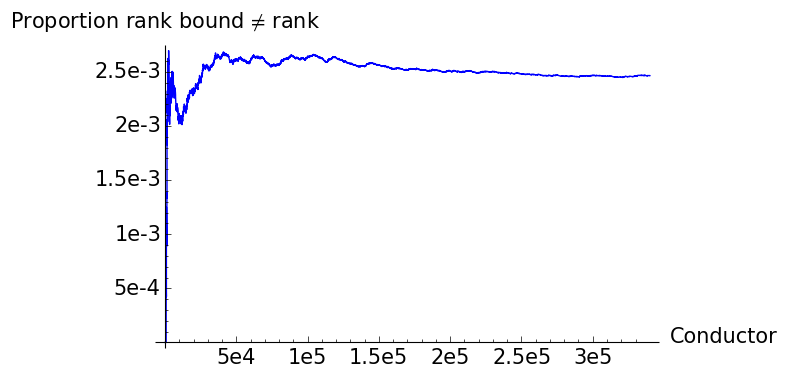
\includegraphics[width=1.0\textwidth]{graphics/rkub_ne_rk.png}
    \caption{The cumulative proportion of curves in the Cremona database for which the sinc$^2$ rank bound was not within 2 of the true rank of the curve, using the scaling $\Delta(E) = \frac{1}{\pi}\left(-\eta + \log\left(\frac{\sqrt{N_E}}{2\pi}\right)\right)$. }
    \label{fig:rkub_ne_rk}
\end{figure}

To generate Figure \ref{fig:rkub_ne_rk}, we used the scaling $\Delta(E) = \frac{1}{\pi}\left(-\eta + \log\left(\frac{\sqrt{N_E}}{2\pi}\right)\right)$, and computed rank bounds on the entire Cremona database of all rational elliptic curves up to conductor 350000; this scaling was chosen so that the bias coming from the first term in the sinc$^2$ sum was always exactly $1$. It was found that the resulting bounds were within 2 of the true rank in 99.75\% of cases. The 4000 or so curves for which the bound exceeded $r_E+2$ all possess anomalously low-lying zeros that 'look like central zeros' when small values of $\Delta$ are used. \\

Since the number of terms in the $c_n$ sum in Equation \ref{eqn:sincsquared_sum} is $e^{2\pi\Delta}$, choosing $\Delta(E) = \alpha \cdot \log N_E$ means that the evaluating the sum will have $\softO\left((N_E)^{2\pi \alpha} \right)$ runtime. That is, the scaling choice used to generate Figure \ref{fig:rkub_ne_rk} yielded an $\softO(N_E)$ computation time. In general, runtime can be made to be $\softO\left((N_E)^{\epsilon}\right)$ for any $\epsilon>0$, at the expense of lowering the fidelity of the bound. \\

It is worth noting explicitly that the accuracy of the sinc$^2$ sum rank estimate is sensitive to low-lying zeros. Thus if it known a priori that the $L$-function of a particular curve does not have any low-lying zeros, a smaller value of $\Delta$ can be used. This fact is exploited in \cite{Bob-2011}, where Bober uses the method on curves of very large rank. There is a well-known phenomenon of zero repulsion in $L$-functions -- zeros tend not to fall as close to each other as could be expected if they were distributed purely randomly on the critical line -- and as such curves with large rank tend to have lowest zeros significantly higher up in the upper half plane than would be expected otherwise. \\

This, for example, allowed Bober to use a $\Delta$ value of only $3.2$ to show that a curve with 28 independent points had analytic rank at most 30. The conductor of the curve in question is roughly $3.4\times 10^{141}$, so using the scaling $\Delta(E) = \frac{1}{\pi}\left(-\eta + \log\left(\frac{\sqrt{N_E}}{2\pi}\right)\right)$ would require a $\Delta$ value of about $51.1$. \\

A related question we can of course ask is: how large does $\Delta$ have to be for the $\sinc^2$ sum rank bound to have perfect fidelity, i.e. guaranteed to be less than $1$ more than the rank of $E$? We will answer this question at the end of section \ref{sec:bite}, though in a way that requires knowledge of an extra invariant attached to $E$, namely the bite $\beta_E$.

\newpage
%%%%%%%%%%%%%%%%%%%%%%%%%%%%%%%%%%%%%%%%%%%%%%%%%%%%%%%%
\section{The Distribution of Nontrivial Zeros}

Though not necessary to prove Equation \ref{eqn:sincsquared_sum}, we may also use zero sums to provide bounds on the density and estimates on the distribution and expected location of the nontrivial zeros of $\Les$ as a function of the curve's conductor.

%%%%%%%%%%%%%%%%%%%%%%%%%%%
\subsection{Explicit Bounds on Zero Density on the Critical Line}

We start by investigating the density of zeros on the critical line. We will see that zero density scales with $\log N_E$; because the explicit formula is used extensively in this section, all results are of course taken to be contingent on GRH. \\

To this end, we define the {\it zero counting function}, which counts the number of zeros on the critical line up to a given bound:
\begin{definition}\label{defn:zero_counting_function}
For non-negative $t$, let $M_E(t)$ be the modified non-trivial zero counting function for $\Les$, i.e.
\begin{equation}
M_E(t) := \sideset{}{\pr}\sum_{|\gamma| \le t} \frac{1}{2},
\end{equation}
where $\gamma$ runs over the imaginary parts of nontrivial zeros of $L_E(s)$, and the prime indicates that the final $\gamma$ is taken with half weight if $\gamma = t$. The central zero is taken with with multiplicity $r_E$, where $r_E$ is the analytic rank of $E$.
\end{definition}

Note that $M_E(0) = \frac{r_E}{2}$, and the function jumps by 1 across the locations of nontrivial zeros, since noncentral zeros come in conjugate pairs and (by GRH) are always simple. \\

%
%Equation \ref{eqn:zero_density} gives us an accurate-up-to-$O(\log t)$ estimate for the number of zeros of $\Les$ on the critical line with imaginary part at most $t$ in magnitude. However, it is also useful to have explicit bounds on the number of zeros in a given interval on the critical line. The results in this section are therefore of course contingent on GRH. \\

We may obtain bounds on $M_E(t)$ via the shifted completed logarithmic derivative $\ldLam{1+s}$. Our workhorse theorem places tight constraints on the sum $\sum_\gamma \frac{\sigma}{\sigma^2+(\gamma-\tau)^2}$ for positive $\sigma$ and real $\tau$. This is a shifted Cauchy distribution-type sum, giving us information on the density of zeros with imaginary part near $\tau$.
\begin{theorem}[GRH]
\label{thm:poisson_sum_bound}
Let $E$ be an elliptic curve with conductor $N_E$ and L-function $L_E(s)$. Let $\sigma > \frac{1}{2}$ and $\tau \in \RR$, and let $\gamma$ range over the imaginary parts of the nontrivial zeros of $L_E(s)$. Then
\begin{equation}
 \left| \sum_\gamma \frac{\sigma}{\sigma^2+(\gamma-\tau)^2} - \left[\log\left(\frac{\sqrt{N_E}}{2\pi}\right) + \Re\left(\digamma(1+\sigma+i \tau)\right)\right] \right| < - 2\frac{\zeta\pr}{\zeta}\left(\frac{1}{2}+\sigma\right).
\end{equation}
\end{theorem}

\begin{proof}
Let $s = \sigma + i \tau$. By equations \ref{eqn:logderiv_relation} and \ref{cor:Re_logderiv} we have
\begin{align*}
\sum_{\gamma} \frac{\sigma}{\sigma^2+(\gamma-\tau)^2} &= \Re\left(\ldLam{1+s}\right) \\
&= \log\left(\frac{\sqrt{N_E}}{2\pi}\right) + \Re\left(\digamma(1+\sigma+i \tau)\right) + \Re\left(\sum_n c_n n^{-s}\right).
\end{align*}
But by lemma \ref{lem:ldLe_bound}
\begin{equation*}
\left|\Re\left(\sum_n c_n n^{-s}\right)\right| \le \left|\ldLe{1+s}\right| < - 2\frac{\zeta\pr}{\zeta}\left(\frac{1}{2}+\sigma\right),
\end{equation*}
so
\begin{equation*}
\left|\sum_\gamma \frac{\sigma}{\sigma^2+(\gamma-\tau)^2} - \log\left(\frac{\sqrt{N_E}}{2\pi}\right) - \Re\left(\digamma(1+\sigma+i \tau)\right)\right| < - 2\frac{\zeta\pr}{\zeta}\left(\frac{1}{2}+\sigma\right).
\end{equation*}
\end{proof}
Note that $\frac{\zeta\pr}{\zeta}$ decays rapidly with increasing $\sigma$, i.e. we have
\begin{equation*}
\sum_\gamma \frac{\sigma}{\sigma^2+(\gamma-\tau)^2} - \left[\log\left(\frac{\sqrt{N_E}}{2\pi}\right) + \Re\left(\digamma(1+\sigma+i \tau)\right)\right] = O(\sigma^{-c})
\end{equation*}
for any $c>0$. \\

\begin{corollary}[GRH]\label{cor:zero_density}
Let $M_E(t)$ be the zero counting function as given in Definition \ref{defn:zero_counting_function}. Then for $t \ge 1$ we have
\begin{equation}
M_E(t) \le t\log N_E +2t\log(t+1).
\end{equation}
If we restrict to $t>~1.32$ we may further simplify this to
\begin{equation}
M_E(t) \le t\log N_E +2t\log t.
\end{equation}
\end{corollary}
\begin{proof}
Take the right inequality in Theorem \ref{thm:poisson_sum_bound} with $\sigma = t$ and $\tau=0$, yielding
\begin{equation*}
\sum_{\gamma} \frac{t}{t^2+\gamma^2} \le \frac{1}{2}\log N_E - \log 2\pi + \digamma(1+t) - 2\frac{\zeta\pr}{\zeta}\left(\frac{1}{2}+t\right),
\end{equation*}
since the digamma function is real on the real axis. \\

Note that for $t \ge 1$ we have $-\frac{\zeta\pr}{\zeta}\left(\frac{1}{2}+t\right) < -\frac{\zeta\pr}{\zeta}\left(\frac{3}{2}\right) = 1.50523\ldots$, since $-\frac{\zeta\pr}{\zeta}$ is decreasing with increasing $t$. Observe that this does not exceed $\log 2\pi = 1.83787\ldots$  \\

Now $\digamma(1+t) < \log(1+t)$ for $t\ge0$. For the second inequality in the theorem, note that $-\frac{\zeta\pr}{\zeta}\left(\frac{3}{2}\right) - \log 2\pi = 0.33264\ldots$, and $\digamma(1+t) \le \log(t) + 0.33264\ldots$ when $t\ge 1.32255\ldots$ \\

Finally, we have that $\sum_{\gamma} \frac{t}{t^2+\gamma^2} \ge \frac{1}{2t}M_E(t)$, since all zeros in the interval $[-t,t]$ are counted with weight at least $\frac{1}{2t}$. Combining the above observations and collecting constants completes the proof.
\end{proof}

It is also useful to have an upper bound on the number of zeros in a given unit interval on the critical line.
\begin{corollary}[GRH]\label{cor:zeros_on_unit_interval}
For $t\ge1$, $M_E(t+1)-M_E(t)$ gives the number of zeros $\gamma$ with $t < |\Im(\gamma)| \le t+1$. We have
\begin{equation}\label{eqn:zeros_on_unit_interval}
M_E(t+1)-M_E(t) < \frac{5}{4}\log(N_E) + \frac{5}{2}\log(t+1).
\end{equation}
\end{corollary}
\begin{proof}
Proceed as before, but now taking the right inequality in theorem \ref{thm:poisson_sum_bound} with $\sigma = 1$ and $\tau=t+\frac{1}{2}$. Observe that
\begin{equation*}
\sum_{\gamma}\frac{1}{1+\left(\gamma-t-\frac{1}{2}\right)^2} \ge \frac{4}{5}\cdot\frac{\left(M_E(t+1)-M_E(t)\right)}{2},
\end{equation*}
since we are only counting zeros in the upper half plane. Also note that similar to before,\\
$\digamma\left(\frac{3}{2}+i\left(t+\frac{1}{2}\right)\right) - \log 2\pi - 2\frac{\zeta\pr}{\zeta}\left(\frac{3}{2}\right) < \log(t+1)$ for $t \ge 1$.
\end{proof}
In a similar manner we derive for $t \ge 1$ that
\begin{equation}\label{eqn:zeros_in_unit_ball}
\#\set{\gamma:\;|\gamma-t|\le 1} < \log(N_E) + 2\log(t+1)
\end{equation}
(note that unlike equation \ref{eqn:zeros_on_unit_interval}, the above only considers zeros with non-negative imaginary part). \\

Finally, recall the definition of the bite of $E$: $\beta_E = \sum_{\gamma \ne 0} \frac{1}{\gamma^2}$. We may use \ref{thm:poisson_sum_bound} to place an explicit bound on the tail end of the inverse square sum via the following:
\begin{corollary}[GRH]\label{cor:sum_tail_bound}
For $\sigma \ge 1$ and $\tau \in \RR$ we have
\begin{equation}
\sum_{|\gamma-\tau|>\sigma} \frac{1}{(\gamma-\tau)^2} \le \frac{\log(N_E) + 2\log(|\tau|+1)}{\sigma}.
\end{equation}
Specifically, when $\tau=0$ we have
\begin{equation}
\sum_{|\gamma|>\sigma} \frac{1}{\gamma^2} \le \frac{\log(N_E)}{\sigma}.
\end{equation}
\end{corollary}
\begin{proof}
Observe that
\begin{equation*}
\frac{\sigma}{2}\cdot\sum_{|\gamma-\tau|>\sigma} \frac{1}{(\gamma-\tau)^2} \le \sum_{|\gamma-\tau|>\sigma} \frac{\sigma}{\sigma^2+(\gamma-\tau)^2} \le\sum_{\gamma} \frac{\sigma}{\sigma^2+(\gamma-\tau)^2},
\end{equation*}
and the rightmost sum is bounded by $\frac{1}{2}\log N_E + \log(|\tau|+1)$ as in the work above. \\
\end{proof}

Equation \ref{thm:poisson_sum_bound} may also used to put lower bounds on the above quantities in some cases, which we hope to pursue in future work.

\newpage
%%%%%%%%%%%%%%%%%%%%%
\subsection{The Expected Number of Zeros up to $t$}

Corollary \ref{cor:zero_density} gives us explicit bounds on zero density, but the bound of $t \log N_E$ is not tight: empirically we see $M_E(t)$ grow more like $\frac{t}{2}\log N_E$; i.e. a factor of $2$ slower. We may again use the explicit formula to come up with a more accurate expansion for the zero counting function, at the expense of have a more nebulous error term that resists attempts to put explicit bounds on it.

\begin{proposition}[GRH]
We have
\begin{equation}\label{eqn:M_E(t)}
M_E(t) = \frac{1}{\pi}\left[\left(-\eta+\log\left(\frac{\sqrt{N_E}}{2\pi}\right)\right) t + \sum_{k=1}^{\infty} \left(\frac{t}{k} - \arctan\left(\frac{t}{k}\right)\right) + \sum_{n=1}^{\infty} \frac{c_n}{\log n}\cdot \sin(t\log n)\right].
\end{equation}
Convergence on the RHS is pointwise with respect to $t$ for both sums; for fixed $t$ convergence for the sums over $k$ and $n$ is absolute and conditional respectively (and {\it extremely} slow for the latter).
\end{proposition}

\begin{proof}
Observe we may write $M_E(t) = \sum_{\gamma}f_t(\gamma)$, where
\begin{equation}
f_t(x) = \begin{cases} \frac{1}{2}, & |x|<t \\ \frac{1}{4}, & |x| = t \\ 0 & |x|> t. \end{cases}
\end{equation}
Informally, we obtain the above formula by integrating both sides of Equation \ref{eqn:exp_form_3} against $f = f_t(x)$, noting that $\hat{f}_t(y) = \frac{\sin(ty)}{y}$. The integrals in the sum over $k$ give us no issue and we may swap the order of the integral and summation signs, since convergence there is absolute. However, some care must be taken when it comes to the sum over $n$, since here convergence is only conditional. 

Formally, we must write $M_E(t)$ as a path integral of $\ldLam{1+s}$ on the path
\begin{equation*}
\epsilon-it \mapsto \epsilon+it \mapsto -\epsilon+it \mapsto -\epsilon-it \mapsto \epsilon-it
\end{equation*}
for some $\epsilon>0$, and invoke the Cauchy Residue Theorem. We may then shrink $\epsilon$ to zero (assuming GRH) to obtain that the RHS of \ref{eqn:M_E(t)} converges point wise to $M_E(t)$ as $m$ and $n \to \infty$.
\end{proof}

Equation \ref{eqn:M_E(t)} may be though of having two components. The first two terms comprise a smooth part that gives the ``expected number of zeros'' up to $t$; and the trigonometric sum over $n$ comprises the discretization information that yields the zeros' exact values relative to their general expected location. We expect the trigonometric sum to be zero infinitely often, and asymptotically it should be positive as often as it is negative. As such the sum should average out to zero and shouldn't contribute any asymptotic bias to the density of zeros on the critical line. We can therefore talk in a real sense of the expected number of zeros up to $t$, which is given by
\begin{equation}\label{eqn:M_E_smooth_part}
\frac{1}{\pi}\left[\left(-\eta+\log\left(\frac{\sqrt{N_E}}{2\pi}\right)\right) t + \sum_{k=1}^{\infty} \left(\frac{t}{k} - \arctan\left(\frac{t}{k}\right)\right)\right].
\end{equation}

Moreover, the trigonometric sum should grow very slowly with $t$. Put more formally, we have the following:
\begin{conjecture}[GRH]\label{conj:trig_sum_size}
GRH implies that
\begin{equation}
\sum_{n=1}^{\infty} \frac{c_n}{\log n}\cdot \sin(t\log n) = O(\log t).
\end{equation}
\end{conjecture}

\begin{figure}[!h]
    \centering
    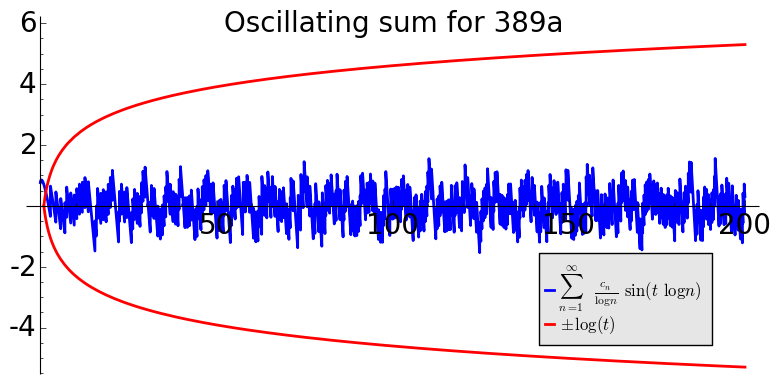
\includegraphics[width=1.0\textwidth]{graphics/M_E_trig_sum_bounds.png}
    \caption{The oscillating sum $\sum_{n=1}^{\infty} \frac{c_n}{\log n}\cdot \sin(t\log n)$ for the curve with Cremona label $389a$ (with equation $y^2 + y = x^3 + x^2 - 2x$) versus $\pm \log(t)$ for $0\le t \le 200$. Numerically we actually see the maximum value of the sum grow slower than $\log(t)$ - possibly $\log(t)^{\alpha}$ for some $0<\alpha<1$, or even $\log\log(t)$.}
    \label{fig:M_E_trig_sum_bounds}
\end{figure}

We won't say much more about bounding the error term in this thesis (or attempt to prove anything about its magnitude), since it requires more advanced analytical tools not mentioned or developed here. \\

\begin{lemma}\label{lem:arctan_sum_size}
For $t \gg 0$, 
\begin{equation}
\sum_{k=1}^{\infty} \left(\frac{t}{k} - \arctan\left(\frac{t}{k}\right)\right) = t\log t + (\eta-1)t + \frac{\pi}{4} + O\left(\frac{1}{t}\right),
\end{equation}
where $\eta = 0.5772\ldots$ is the Euler-Mascheroni constant.
\end{lemma}
\begin{proof}
We have
\begin{equation*}
\sum_{k=1}^{\infty} \left(\frac{t}{k} - \arctan\left(\frac{t}{k}\right)\right) = \int_{0}^{t} \sum_{k=1}^{\infty} \frac{x^2}{k(k^2+x^2)} \; dx = \int_{0}^{t} \Re\left(\digamma(1+ix) + \eta\right) \; dx,
\end{equation*}
where $\digamma(z)$ is the digamma function on $\CC$. Now along the critical line we have the following asymptotic expansion for the real part of the digamma function:
\begin{equation}
\Re\left(\digamma(1+ix)\right) = \log x + \frac{1}{12} x^{-2} + O(x^{-4})
\end{equation}
Hence $\int_{0}^{t} \Re\left(\digamma(1+ix)\right) \; dx = t(\log t - 1)  + O(1)$. The constant term of $\frac{\pi}{4}$ comes from integrating the difference between $\Re\left(\digamma(1+ix)\right)$ and $\log x$ between $0$ and $\infty$:
\begin{equation*}
\int_{0}^{\infty} \left[\Re\left(\digamma(1+ix)\right) - \log x\right] \; dx = \frac{\pi}{4}.
\end{equation*}
The result follows.
\end{proof}

Conjecture \ref{conj:trig_sum_size} and lemma \ref{lem:arctan_sum_size} combine to give us a precise asymptotic statement on the distribution of zeros up to $t$, in the same vein as von Mangoldt's asymptotic formula for the number of zeros up to $t$ for $\zeta$:

\begin{theorem}[GRH]\label{thm:zero_density}
Let $E$ have conductor $N_E$. Then for $t\gg0$ we have
\begin{equation}\label{eqn:zero_density}
M_E(t) = \frac{t}{\pi} \, \log\left(\frac{t\sqrt{N_E}}{2\pi e}\right) + \frac{1}{4} + O(\log t),
\end{equation}
where the error term is positive as often as it negative and contributes no net bias.
\end{theorem}

\begin{figure}[!h]
    \centering
    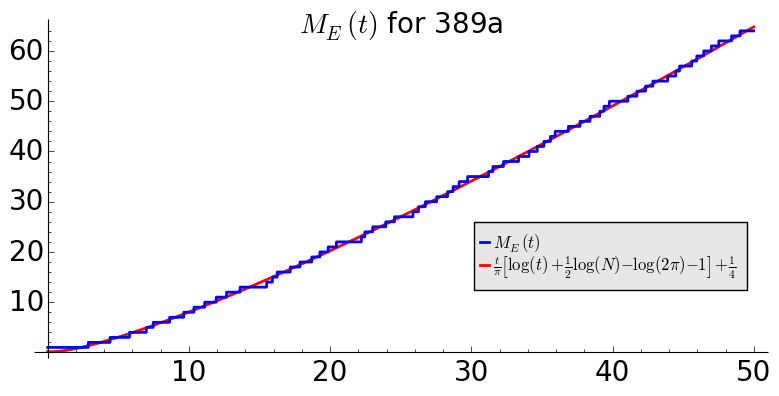
\includegraphics[width=1.0\textwidth]{graphics/M_E_389.png}
    \caption{The number of zeros up to $t$ versus $\frac{t}{\pi}\left[\log\left(\frac{t\sqrt{N_E}}{2\pi}\right) -1 \right] + \frac{1}{4}$ for the Cremona curve $389a$. The match up is extremely good.}
    \label{fig:M_E_389}
\end{figure}

\begin{corollary}[GRH]
For $t\gg0$, the number of zeros on the critical line in a unit interval
\begin{equation}
M_E(t)-M_E(t-1) = \frac{1}{\pi}\log\left(\frac{t\sqrt{N_E}}{2\pi}\right) + O(\log t),
\end{equation}
where again the error term contributes no net bias.
\end{corollary}

That is, zero density on the critical line grows like $\frac{1}{2}\log N_E + \log t$, where $N_E$ is the conductor of $E$ and $t$ the distance from the real axis. \\

Neglecting the oscillating error term in Equation \ref{eqn:zero_density}, we may solve for $t$ in terms of the Lambert $W$-function to obtain an explicit formula for the expected value of the imaginary part of the $n$th zero on the critical line. Recall the definition of the Lambert $W$-function: if $y = x e^x$, then $x = W(y)$. $W$ is a multiple-valued function; we make use of the principle branch $W_0$ below:
\begin{corollary}[GRH]\label{cor:gamma_n_approx_value}
Let $\gamma_n := \gamma_n(E)$ be the imaginary value of the $n$th nontrivial (and noncentral) zero in the upper half plane of $\Les$ with analytic rank $r_E$. Then
\begin{equation}\label{approx:gamma_n}
\gamma_n \sim \frac{2\pi e}{\sqrt{N_E}} \cdot \exp \left(W_0\left[\left(\frac{r_E}{2} +n - \frac{3}{4}\right)\cdot \frac{\sqrt{N_E}}{2 e}\right]\right),
\end{equation}
in the sense that for a given curve, the difference between the above value and the true value of $\gamma_n$ will on average be zero as $n \to \infty$.
\end{corollary}
\begin{proof}
Observe that the $n$th nontrivial noncentral zero has imaginary part $t$ when $M_E(t) = \frac{r}{2} + n - \frac{1}{2}$ (since the final zero is counted with half weight). Hence using Equation \ref{eqn:zero_density} sans the oscillating error term, we solve for $t$ in
\begin{equation*}
\frac{t}{\pi} \, \log\left(\frac{t\sqrt{N_E}}{2\pi e}\right) + \frac{1}{4} = \frac{r_E}{2} + n - \frac{1}{2}.
\end{equation*}
\end{proof}

[Aside: The principle branch of the Lambert $W$-function has the asymptotic expansion $W_0(x) = \log x - \log \log x + o\left(1\right)$, for $n \gg 0$ we recover the known asymptotic for the location of the $n$th nontrivial zero: $\gamma_n = O\left(\frac{n}{\log n} \right)$. Better yet, after some manipulation the asymptotic expansion gives us the proportionality constant explicitly:
\begin{equation}
\lim_{n \to \infty} \frac{\gamma_n}{\frac{n}{\log n}} = \pi.
\end{equation}
Note, however, that the convergence rate is slow: $O(\frac{1}{\log n})$, and the constant in front scales with the log of the conductor of $E$.] \\

A natural question to ask, given that we now have an expected value for $\gamma_n$, is: how much does the imaginary part of the $n$th zero deviate from its expected location? To this end we define the {\it dispersion} of the $n$th zero:
\begin{definition}
The dispersion $\delta_n(E) := \delta_n$ of the imaginary part of the $n$th nontrivial zero in the upper half plane is the difference between the true and predicted values of $\gamma_n$, i.e.
\begin{equation}
\delta_n = \gamma_n - \frac{2\pi e}{\sqrt{N_E}} \cdot \exp \left(W_0\left[\left(\frac{r_E}{2} +n - \frac{3}{4}\right)\cdot \frac{\sqrt{N_E}}{2 e}\right]\right).
\end{equation}
\end{definition}

\begin{figure}[!h]
    \centering
    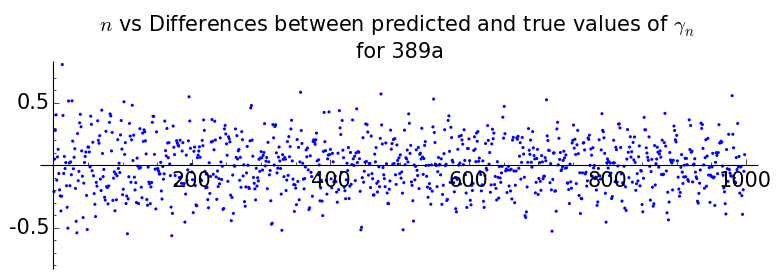
\includegraphics[width=1.0\textwidth]{graphics/389a_zero_dispersions_scatterplot.png}
    \caption{A scatter plot of zero dispersions for the first 1000 nontrivial zeros of the Cremona curve 389a, the rank 3 curve with smallest conductor. The values are seldom more than $\frac{1}{2}$.}
    \label{fig:389a_zero_dispersions_scatterplot}
\end{figure}

\begin{figure}[!h]
    \centering
    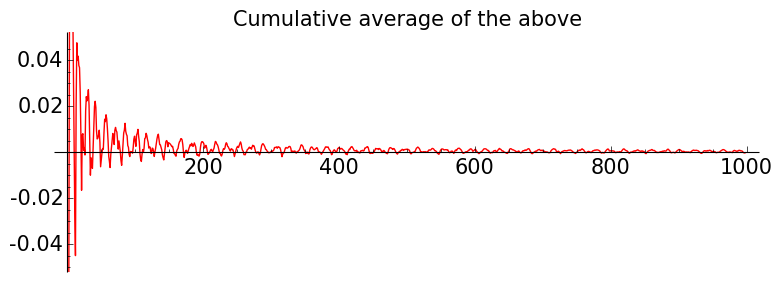
\includegraphics[width=1.0\textwidth]{graphics/389a_zero_dispersions_cumulative_average.png}
    \caption{A cumulative average plot of the above, showing clearly that asymptotically, the average difference between the predicted and true values of $\gamma_n$ is zero. The positive bias at the beginning comes from the $O(1/t)$ term in Lemma \ref{lem:arctan_sum_size}. Interestingly, although the deviations might a priori appear completely random, there is a clear oscillating structure in the average, and the line about which the oscillation occurs appears to decrease to zero from above.}
    \label{fig:zero_dispersions_cumulative_average}
\end{figure}

Even though the above graph demonstrates that the zero dispersions are clearly not random, when viewed as a i.i.d. time series, the dispersions appear be normally distributed. \\

\begin{figure}[!h]
    \centering
    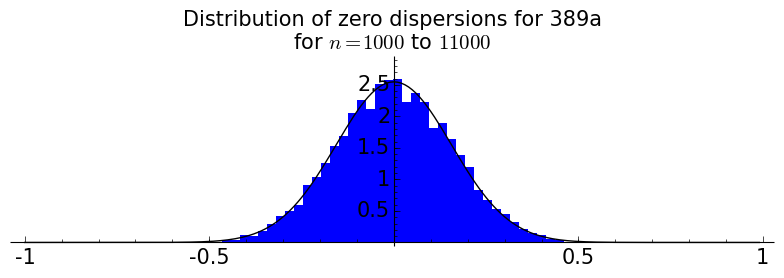
\includegraphics[width=1.0\textwidth]{graphics/389a_zero_dispersions_histagram.png}
    \caption{A histogram of zero dispersions for the curve 389 for the 1000th through 11000th zeros (we discard the first 1000 zeros to avoid the small-height bias observable in the cumulative average plot above). }
    \label{fig:389a_zero_dispersions_histagram}
\end{figure}

For the data set used the graph above, the mean was $3.16\times10^{-5}$ (a good indicator that the expected value formula contains no systematic bias), standard deviation $0.1566$. The standard deviation appears to decrease with increasing $n$: we applied the Shapiro-Wilk normality test on batches of 1000 consecutive zero dispersions, and got $p$-values in excess of $0.2$ (and most of the time in excess of 0.5) in all cases. Moreover, the computed standard deviations decreased uniformly from $0.1745$ for the $n=1000$ to $2000$ dispersion set, to $0.1464$ in the $n=10000$ to $11000$ set. We hope to pursue this investigation in future work. \\

Finally, we may also go in the other direction and use Equation \ref{eqn:M_E(t)} to make a guess as to the expected imaginary part of the {\it lowest} noncentral nontrivial zero of $\Les$ as a function of increasing conductor $N_E$:
\begin{proposition}[GRH]
For a curve $E$ with large conductor $N_E$ and analytic rank $r_E$, the best guess for the imaginary part of the first nontrivial noncentral zero $\gamma_0$ of $\Les$ in the upper half plane is
\begin{equation}
\gamma_0 = \frac{(r_E+1)\pi}{\log(N_E) -2\log(2\pi) -2\eta}.
\end{equation}
\end{proposition}
The derivation is similar to before. The location of the first nontrivial noncentral zero is given by the value of $t$ for which $M_E(t)$ jumps from $r_E/2$ to $r_E/2+1$; at that point $M_E(t) = r_E/2 + 1/2 = \frac{r_E+1}{2}$, so the expected value of $\gamma_1$ is given by setting equation \ref{eqn:M_E(t)} equal to $\frac{r_E+1}{2}$ and solving for $t$. \\

Now, however, $\frac{1}{\pi}\sum_{k=1}^{\infty} \left[\frac{t}{k} - \arctan\left(\frac{t}{k}\right)\right]$ is $O(t^3)$ for small t, so the quantity expressed in equation \ref{eqn:M_E_smooth_part} is dominated by the $\frac{1}{\pi}\left(-\eta+\log\left(\frac{\sqrt{N_E}}{2\pi}\right)\right) t$ term when $N_E$ is large. Solving for $t$ yields the desired value.

\newpage
%%%%%%%%%%%%%%%%%%%%%%%%%%%%%%%%%%%%%%%%%%%%%%%%%%%%%%
\section{The Bite}\label{sec:bite}

Mazur and Stein in \cite{MaSt-2013} define the {\it bite} of an elliptic curve:
\begin{definition}\label{defn:bite}
The {\it bite} of $\Les$ is
\begin{equation}
\beta(E) := \sum_{\gamma \ne 0} \gamma^{-2},
\end{equation}
where the sum runs over the imaginary parts of all {\it noncentral} nontrivial zeros of $\Les$.
\end{definition}
This quantity is of interest for a variety of reasons: it controls the rate of convergence in many explicit formula-type sums for $\Les$, and is intimately linked with the analytic rank and leading central Taylor coefficient for the $L$-series of $E$. Again, the explicit dependence on $E$ may be left as understood if the choice of $E$ is unambiguous, or we may subsume the dependence on $E$ into a subscript and write $\beta_E$. In this final section we establish some bounds involving the bite, show how one can compute it efficiently without having to compute the locations of the zeros of $\Les$ explicitly, and give some zero sum examples relevant to this thesis where the bite comes into play. \\

Since sums of inverse higher powers of zeros also crop up, we generalize the notion of bite as follows:
\begin{definition}
For positive integer $n$, the {\it higher order bite} of order $n$ for $\Les$ is
\begin{equation}
\beta_n(E) := \sum_{\gamma \ne 0} \gamma^{-n}.
\end{equation}
\end{definition}
Thus $\beta_2(E) = \beta_E$ as defined previously. Note also that $\beta_n = 0$ for any odd $n$, since zeros come in conjugate pairs. \\

Equation \ref{eqn:ldLam_sum} gives us a description of the Laurent expansion of $\ldLam{1+s}$ about zero:
\begin{proposition}[GRH]\label{prop:ldLam_series_at_zero}
The Laurent expansion of $\ldLam{1+s}$ about zero is given by
\begin{align}
\ldLam{1+s} &= \frac{r_E}{s} + \beta_2\cdot s - \beta_4\cdot s^3 + \beta_6\cdot  s^5 - \ldots \\
& = \frac{r_E}{s} + \sum_{k=1}^{\infty} (-1)^{k-1}\beta_{2k}\cdot s^{2k-1},
\end{align}
and this converges for $|s|<\gamma_0$, where $\gamma_0$ is the imaginary part of the lowest noncentral nontrivial zero of $\Les$ in the upper half plane.
\end{proposition}
The proof of this follows immediately by expanding the sum in Equation \ref{eqn:ldLam_sum} and collecting terms. \\

\begin{corollary}[GRH]\label{cor:ldLe_expansion}
Let $E/\QQ$ have conductor $N_E$, $L$-function $\Les$ with bite $\beta_E = \beta_2(E)$ and central leading coefficient $C_E\pr$. Let the Taylor series expansion of $L_E$ about the central point be
\begin{equation}
L_E(1+s) = C_E\pr \, s^{r_E}\left[1 + a\cdot s + b\cdot s^2 + O(s^3)\right]
\end{equation}
Then 
\begin{align}
a &= -\left[-\eta + \log\left(\frac{\sqrt{N_E}}{2\pi}\right)\right] \\
2b &= \left[-\eta + \log\left(\frac{\sqrt{N_E}}{2\pi}\right)\right]^2 - \frac{\pi^2}{6} + \beta_E,
\end{align}
where $\eta$ is the Euler-Mascheroni constant $= 0.5772\ldots$.
\end{corollary}

\begin{proof}
We note that the digamma function has the following Taylor expansion about $s=1$:
\begin{equation}
\digamma(1+s) = -\eta - \sum_{k=1}^{\infty} (-1)^k \zeta(k+1) s^k,
\end{equation}
where $\eta$ is the Euler-Mascheroni constant, and $\zeta(s)$ is the Riemann zeta function. \\
Thus by equation \ref{eqn:logderiv_relation} and Proposition \ref{prop:ldLam_series_at_zero} we have that
\begin{equation*}
\ldLe{1+s} = \frac{r_E}{s} - \left[-\eta + \log\left(\frac{\sqrt{N_E}}{2\pi}\right)\right] + \left[-\zeta(2) + \sum_{\gamma\ne0} \gamma^{-2}\right]\cdot s + O(s^2).
\end{equation*}
But if $L_E(1+s) = C_E\pr \, s^{r_E}\left[1 + a\cdot s + b\cdot s^2 + O(s^3)\right]$, then careful logarithmic differentiation yields
\begin{equation*}
\ldLe{1+s} = \frac{r_E}{s} + a + \left(-a^2 + 2b\right)\cdot s + O(s^2).
\end{equation*}
Comparing terms and solving for the relevant quantities produces the desired formulae.
\end{proof}
We may continue in the same vein to produce formulae for higher order coefficients of $L_E(s)$. As can be seen from above, these can in general be written in terms of sums of powers of the quantity $\left[-\eta + \log\left(\frac{\sqrt{N_E}}{2\pi}\right)\right]$ (which is the constant term in the Laurent series of $\ldLam{1+s}$), inverse sums of even powers of the nontrivial zeros, and $\zeta(n)$ for $n$ a positive integer. \\

In other words, $\beta_E$ and higher-order bites encode information about higher order terms in the Taylor expansion of $L_E(1+s)$; moreover, the Taylor series thereof contains no new information about the curve's attached invariants beyond that which can be found in the first nonzero coefficient and the bites $\beta_{2n}(E)$. Whether the bites do indeed have any arithmetic significance, however, is an open question. \\

As can be seen from the above, the bite of a curve is of interest is due to it being intimately linked with the leading central Taylor coefficient $C_E$ of $\Lambda_E(1+s)$ and the (analytic) rank $r_E$. We may link the three quantities explicitly with a suite of inequalities derived from point estimates on the $L$-function of $E$ and the logarithmic derivative thereof. First, we will need the following technical lemma:
\begin{lemma}[GRH]\label{lem:bite_rank_sigma_inequality}
Let $\sigma > \frac{1}{2}$. The bite $\beta_E$ and analytic rank $r_E$ of a curve $E$ obey
\begin{equation}
\sigma \cdot \beta_E + \frac{r_E}{\sigma} > \frac{1}{2} \log N_E + \digamma(1+\sigma)-\log(2\pi) - 2\frac{\zeta\pr}{\zeta}\left(\frac{1}{2}+\sigma\right),
\end{equation}
where $\digamma(s) = \frac{\Gamma\pr}{\Gamma}(s)$ is the digamma function on $\CC$, $\zeta(s)$ is the Riemann zeta function and $N_E$ is the conductor of $E$.
\end{lemma}
\begin{proof}
From Equation \ref{thm:poisson_sum_bound}, letting $\tau=0$, we get
\begin{equation}
\sum_\gamma \frac{\sigma}{\sigma^2+\gamma^2} > \log\left(\frac{\sqrt{N_E}}{2\pi}\right) + \digamma(1+\sigma) - 2\frac{\zeta\pr}{\zeta}\left(\frac{1}{2}+\sigma\right).
\end{equation}
But
\begin{align*}
\sum_\gamma \frac{\sigma}{\sigma^2+\gamma^2} &= \frac{1}{\sigma} \sum_\gamma \frac{1}{1+\left(\frac{\gamma}{\sigma}\right)^2} \\
&< \frac{1}{\sigma}\left(r_E + \sum_{\gamma\ne 0} \frac{1}{\left(\frac{\gamma}{\sigma}\right)^2} \right) \\
&= \frac{r_E}{\sigma} + \sigma\cdot \beta_E.
\end{align*}
Combining inequalities completes the proof.
\end{proof}

We then have the following:
\begin{proposition}[GRH]\label{prop:beta_C_r_bounds}
Let $\beta_E$, $C_E$, $r_E$ and $N_E$ be the bite, completed $L$-function leading central Taylor coefficient, analytic rank and conductor of $E$ respectively. Then
\begin{align}
(1+\beta_E)\cdot C_E & < 0.173 \cdot N_E, \\
\beta_E + \log C_E &> \frac{1}{2} \log N_E - 5.229,  \\
\beta_E + r_E & > \frac{1}{2} \log N_E - 4.426.
\end{align}
\end{proposition}
\begin{proof}
The third inequality is a specialization of Lemma \ref{lem:bite_rank_sigma_inequality} with $\sigma=1$, with the conductor-independent terms lumped together into one numerical value. The first two inequalities come from the Hadamard product of the completed $L$-function (Equation \ref{eqn:Lams_prod}) evaluated one unit to the right of the central point:
\begin{equation}
\Lambda_E(2) = C_E\cdot \prod_{\gamma \ne 0} \left(1+\frac{1}{\gamma^2}\right),
\end{equation}
noting that $1+\beta_E < \prod_{\gamma \ne 0} \left(1+\frac{1}{\gamma^2}\right) < e^{\beta_E}$. On the other hand from the definition of the completed $L$-function we have $\Lambda_E(2) = N_E \cdot (2\pi)^{-2}\cdot  L_E(2)$. Inequality \ref{ineq:bounds_on_Les} has that $\frac{\zeta(3)^2}{\zeta(\frac{3}{2})^2} < L_E(2) < \zeta\left(\frac{3}{2}\right)^2$; combining inequalities and collecting constant terms in the respective inequalities completes the two results.
\end{proof}
The take-away from Proposition \ref{prop:beta_C_r_bounds} is that the bite and the leading Taylor coefficient $C_E$ cannot both be very large or very small simultaneously relative to the conductor. Similarly, the larger the rank of a curve, the smaller $\beta_E$ can be relative to $N_E$. \\

We can go even further and establish a lower bound on $\beta_E$ in terms of $N_E$ independent of $C_E$ and $r_E$, at the expense of introducing a non-explicit constant. As asymptotic zero density on the critical line grows proportional to $\log N_E$ (see Theorem \ref{thm:zero_density}), we expect the bite to grow at least like $\log N_E$ too, regardless of the limiting behavior of zeros near the central point. This is indeed the case:
\begin{proposition}[GRH]
For all $\epsilon>0$ there is a constant $K_{\epsilon}>0$ such that for all elliptic curves $E$, the bite of $E$ obeys
\begin{equation}\label{eqn:bite_lower_bound}
\beta_E = \sum_{\gamma\ne 0} \frac{1}{\gamma^2} > \frac{1}{1+\epsilon} \log N_E - K_{\epsilon}.
\end{equation}
where $N_E$ is the conductor of $E$.
\end{proposition}
\begin{proof}
We again invoke Lemma \ref{lem:bite_rank_sigma_inequality} to observe that
\begin{equation}
\beta_E > \frac{1}{2\sigma} \log N_E - \frac{r_E}{\sigma^2} + \frac{1}{\sigma}\left[\digamma(1+\sigma)-\log(2\pi) + 2\frac{\zeta\pr}{\zeta}\left(\frac{1}{2}+\sigma\right)\right],
\end{equation}
where the term in the square brackets is independent of $N_E$ and is finite for any $\sigma>\frac{1}{2}$. By Corollary \ref{cor:rank_slower_than_log_N}, the rank $r_E$ grows slower than any multiple  of $\log N_E$. Hence for $\epsilon > 0$ we may, for example, take $r_E < \epsilon^2 \log N_E + K\pr(\epsilon^2)$ for some constant $K\pr$ dependent on $\epsilon^2$, and then let $\sigma = \frac{1}{2}+\frac{1}{2}\epsilon$. This allows the constant in front of the collected $\log N_E$ term to be made arbitrarily close to 1 from below, while all other terms sum to a finite value independent of $E$.
\end{proof}

In reality we expect the bite to grow faster than $\log N_E$ -- as zero density scales with $\log N_E$, the sum of the inverse squares thereof should na\"{i}vely be expected to grow with $(\log N_E)^2$. However, this is discounting any unusual behaviour of zeros near the central point. Sarnak has mentioned in private correspondence that it's believed that the lowest noncentral zero $\gamma_0$ actually approaches a constant limiting distribution as conductor goes to infinity, which would in turn decrease any lower bound that can be placed on the bite. \\

\begin{figure}[!h]
    \centering
    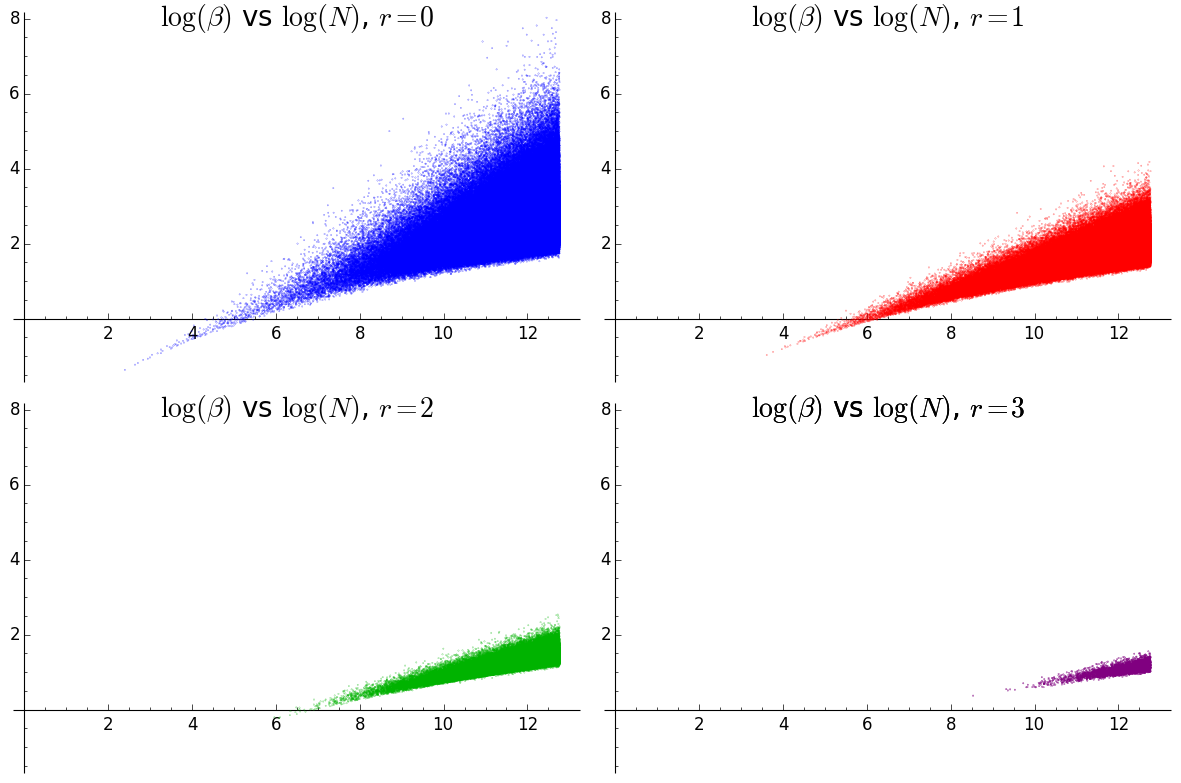
\includegraphics[width=1.0\textwidth]{graphics/bites_vs_conductors_array.png}
    \caption{The bites of all curves in the Cremona tables were computed using the above method. Above is a scatterplot of $\log \beta_E $ vs. $\log N_E$ for curves of rank 0, 1, 2 and 3 respectively. }
    \label{fig:bites_vs_conductors_array}
\end{figure}

One can see from Figure \ref{fig:bites_vs_conductors_array} that the bite obeys a sharp lower bound with respect to the conductor, but the upper bound is somewhat less tight. More interesting is the fact that the lower bound appears the same regardless of rank, while curves with anomalously large bites are predominantly rank $0$. This makes sense: large bites correspond to very low-lying zeros, and because of the well-documented zero repulsion effect, this usually only happens when there are no zeros at the central point. \\

How does one go about computing the bite of an elliptic curve? The na\"{i}ve way would be to compute the location of the $n$ zeros up to some bound and then add up their inverse squares to get an approximation of $\beta_E$. This can indeed be done, for example via Rubinstein's {\tt lcalc} package. However it is slow and inefficient, and one will always introduce some truncation error via this method.  \\

Instead, the following result allows us to relate the bite directly to the leading Taylor coefficient $C_E$ and higher derivatives of $\Lambda_E(s)$ at the central point:
\begin{proposition}[GRH]\label{prop:bite_times_leading_coeff}
Let $E$ have completed $L$-function $\Lams$ and analytic rank $r_E$. Then
\begin{equation}
\beta_E\cdot C_E = \frac{\Lambda_E^{(r_E+2)}(1)}{(r_E+2)!},
\end{equation}
where $\beta_E$ is the bite of $E$, and $C_E$ is the leading coefficient of $\Lams$ at the central point.
\end{proposition}
\begin{proof}
From equation \ref{eqn:Lams_prod} we have that 
\begin{equation}
\Lambda_E(1+s) = C_E\left(s^{r_E} + \beta_E s^{r_E+2} + O(s^{r_E+4})\right).
\end{equation}
Differentiating $r_E+2$ times and evaluating at $s=0$ achieves the desired result.
\end{proof}

It is worth noting explicitly that one cannot hope to be able to compute the bite of a curve without knowing its analytic rank -- we have to know how many zeros are precisely at the central point and not just $\epsilon$ away from the central point, otherwise $\beta_E$ could be arbitrarily large. This obstruction notwithstanding, Proposition \ref{prop:bite_times_leading_coeff} gives us a straightforward way to compute the bite of $E$ from the $r_E$th and $(r_E+2)$th Taylor coefficients of $L_E(1+s)$:
\begin{corollary}[GRH]
\begin{align}\
\beta_E \quad &= \frac{1}{(r_E+1)(r_E+2)} \cdot \frac{\Lambda_E^{(r_E+2)}(1)}{\Lambda_E^{(r_E)}(1)} \label{eqn:bite_via_Lams} \\
&= \frac{2}{(r_E+1)(r_E+2)} \cdot \frac{L_E^{(r_E+2)}(1)}{L_E^{(r_E)}(1)} - \left(-\eta+\log\left(\frac{\sqrt{N_E}}{2\pi}\right)\right)^2 + \frac{\pi^2}{6} \label{eqn:bite_via_L_E}.
\end{align}
\end{corollary}
\begin{proof}
The first line follows immediately from Proposition \ref{prop:bite_times_leading_coeff} and the fact that $C_E = \frac{\Lambda^{(r_E)}(1)}{r_E!}$. The second line comes from the formula for the $(r_E+2)$th Taylor coefficient of $L_E$ at the central point derived in Corollary \ref{cor:ldLe_expansion}.
\end{proof}
We can therefore compute the bite of a curve {\it without} having to compute the locations of the zeros themselves. Moreover, Theorem \ref{thm:main_theorem} implies that the bite can be provably computed to $k$ bits precision in $\softO(k\cdot \sqrt{N_E})$ time (assuming standard conjectures). This may be done, for example, via Tim Dokchitser's {\tt computel} PARI code, which can compute the Taylor series expansion of a motivic $L$-function at a given point. [Important side-note: the aforementioned package uses approximations that have not (yet) been shown to be provably correct; however, one could certainly write code to compute in square root time the central Taylor expansion of $\Les$ via the work of Bradshaw in \cite{Bra-2010}, which {\it does} produce provably correct $L$-function values.] \\

\begin{figure}[!h]
    \centering
    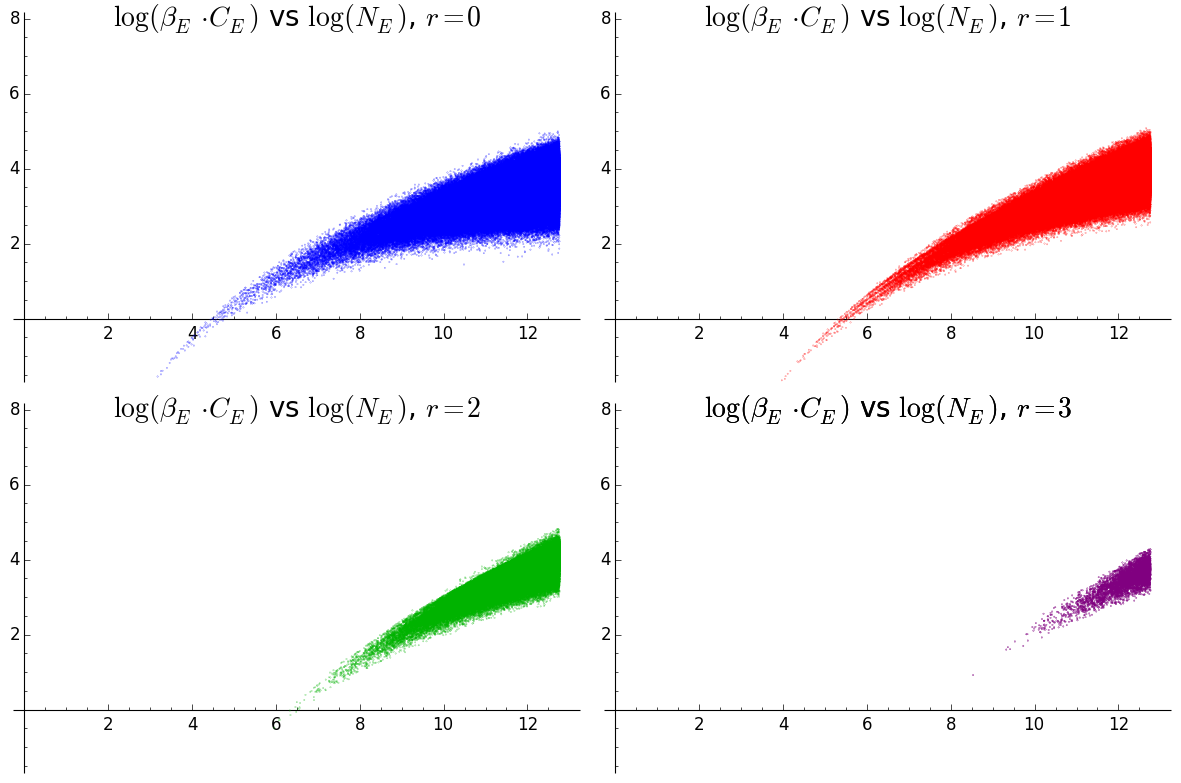
\includegraphics[width=1.0\textwidth]{graphics/beta_times_C_vs_conductors_array.png}
    \caption{A scatter plot of $\log (\beta_E \cdot C_E) $ vs. $\log N_E$ for all curves up to conductor 350000, differentiated by rank. The constrained nature of the quantity $\beta_E \cdot C_E$ is readily apparent. }
    \label{fig:bites_vs_conductors_array}
\end{figure}

We finish off this section with a result giving an indication of one other area in which the bite of a curve comes into play: controlling convergence rates in explicit formula type sums. This is a topic worthy of its own paper, so we shall just present two examples relevant to the work in this thesis.

\begin{theorem}[GRH]\label{thm:sinc_squared_sum_with_bite}
Let $\sum_{\gamma} \sinc^2(\Delta \gamma)$ be the $\sinc^2$ sum for $E$ with parameter $\Delta$, as detailed in Equation \ref{eqn:sincsquared_sum}. If we let $\Delta = \frac{1}{\pi}\cdot \sqrt{\frac{\beta_E}{n}}$, then the sum will evaluate to a value less than than $r_E+n$, where $r_E$ is the analytic rank of $E$.
\end{theorem}
\begin{corollary}[GRH]\label{cor:sinc_squared_sum_with_bite}
The analytic rank of $E$ is the largest integer less than
\begin{equation}\label{eqn:sinc_squared_sum_with_bite}
\frac{1}{\sqrt{\beta_E}}\left[\left(-\eta + \log\left(\frac{\sqrt{N_E}}{2\pi}\right)\right)+ \frac{1}{2 \sqrt{\beta_E}}\left(\frac{\pi^2}{6} - \Li_2\left(e^{-2\sqrt{\beta_E}}\right)\right) + \sum_{\log n<2\sqrt{\beta_E}} c_n \cdot \left(1-\frac{\log n}{2\sqrt{\beta_E}}\right)\right].
\end{equation}
\end{corollary}
\begin{proof}
We note that 
\begin{equation}
\sum_{\gamma} \sinc^2(\Delta \gamma) = r_E + \sum_{\gamma\ne 0} \sinc^2(\Delta \gamma) <  r_E + \sum_{\gamma\ne 0} \frac{1}{(\pi \Delta \gamma)^2} = r_E + \frac{1}{\pi^2 \Delta^2} \cdot \beta_E.
\end{equation}
So choosing $\Delta = \frac{1}{\pi}\cdot \sqrt{\frac{\beta_E}{n}}$ bounds the sum value from above by $r_E + n$. The corollary follows immediately from Equation \ref{eqn:sincsquared_sum} the case with $n=1$.
\end{proof}

This formula comes with one giant caveat that renders it of little use practically -- it requires knowing the bite of a curve, which of course in itself requires knowing the curve's analytic rank a priori. Nevertheless, the above serves to underscore that determining the bite and determining the analytic rank of a curve are computationally equivalent: we can compute the bite knowing the rank via Equations \ref{eqn:bite_via_Lams} or \ref{eqn:bite_via_L_E}, and we can compute the rank knowing the bite via Formula \ref{eqn:sinc_squared_sum_with_bite}. \\

Using the bite we have an even simpler way to compute the analytic rank of an elliptic curve:
\begin{theorem}[GRH]\label{thm:compute_rank_by_logderiv}
\begin{equation}
r_E = \left\lfloor\frac{1}{\sqrt{\beta_E}}\cdot \ldLam{1+\frac{1}{\sqrt{\beta_E}}}\right\rfloor.
\end{equation}
\end{theorem}
\begin{proof}
By Equation \ref{eqn:ldLam_sum}, the Hadamard product expansion of $\ldLam{1+s}$ gives us \begin{equation}
s\cdot \ldLam{1+s} = s\cdot \prod_{\gamma} \frac{s}{s^2+\gamma^2} = r_E + \prod_{\gamma\ne 0} \frac{1}{1+(\frac{\gamma}{s})^2} < r_E + s^2\cdot \beta_E.
\end{equation}
So, analogous to the method used in the proof of Theorem \ref{thm:sinc_squared_sum_with_bite}, evaluating at $s = \sqrt{\frac{n}{\beta_E}}$ gives a real value bounded by $r_E+n$.
\end{proof}

Again, there are subtle issues present with this formula. Apart from again having to know the bite of a curve, even though we can evaluate $\Lambda_E(s)$ and its derivative to any given precision in $\softO(\sqrt{N_E})$ time, the same is not true for the logarithmic derivative. Namely, we may encounter destructive precision loss near the central point if $r_E$ has high analytic rank and/or low-lying zeros. We therefore caution against using this method to determine analytic rank willy-nilly, as in our mind it does {\it not} constitute a method to compute rank provably without doing more work.
